\chapter[MD simulations of PgaB-glucosamine binding]{Molecular Dynamics simulations of PgaB and monosaccharides of N-acetyl-glucosamine and glucosamine}

\emph{Reference}: This work contributed to the manuscript, ``PgaB Contains a Carbohydrate Binding Domain Required for Modification and Export of Poly-$\beta$-1,6-N-acetyl-D-glucosamine", which is to be submitted to PNAS
\\
\\
\emph{Contributions}:
Grace Li conducted the MD simulation part of the research and wrote the section. Dustin Little conducted and interpreted the experimental results. Chris Ing parameterized the partial charges for glucosamine. R\'{e}gis Pom\`{e}s, Lynne Howell, Mark Nitz provided editorial input and guidance.

\newpage

% \section{Summary}
% Note that this summary was taken from a draft of the paper written by Dustin from April 5th, 2013
%Bacteria embedded in a self-produced matrix of exopolymeric substance, or biofilm, are tolerant to antibiotics, protected from the environment, and isolated from the innate immune system. Production and de-N-acetylation of the exopolysaccharide poly-$\beta$-1,6-N-acetyl-D-glucosamine (PNAG) is important for biofilm formation in Escherichia coli. PgaB is essential for the partial de-N-acetylation of PNAG (dPNAG); a process required for polymer export and subsequent biofilm formation. Here we report 1.9 Å crystal structures of PgaB’s isolated C-terminal domain (PgaB-CT) and complex with glucosamine. The structure of PgaB-CT has structural difference from the previously reported PgaB42-655 structure (\textbf{What are these differences?}). Characterization of PgaB-CT using tryptophan fluorescence quenching assays shows binding to PNAG oligomers with ~1-4 mM affinity. These data in combination with molecular dynamics simulations of PgaB with N-acetylglucosamine and glucosamine suggest PNAG de-N-acetylation occurs first, with subsequent binding of dPNAG to the C-terminal domain. We believe this concerted action plays a pivotal role in targeting dPNAG for export through the outer membrane porin PgaA.
%
%From the book chapter XXX, PNAG is a homopolymer of beta(1,6) glcnac but with 20\% of the monomers deacetylated. But then what would be the difference between dPNAG and PNAG? Or is it just a terminology difference between the two?

% \section{Introduction}
% \textbf{In the second paper, experiments were performed to characterize the ability of PgaB-CT domain to bind carbohydrate substrates, which are short oligosaccharides of \pnag. The results of this study suggests a mechanism by which polymer substrates are bound and synthesized onto the protein. Furthermore, a proposed mechanism of export is discussed.}

% \textbf{commentary: From reading what Dustin has written in the current introduction, I think their experimental data is quite weak. Their key result is: ``We show PgaB-CT binds PNAG oligomers with low affinity (what's the range?) using tryptophan fluorescence quenching, and have determined the structure of PgaB-CT in complex with glucosamine.'' I think MD simulations will be their best leverage for the proposed mechanism of export.}

% PgaB - description of the study, motivation and what has been done thus far
% PgaB is a protein required for the partial de-N-acetylation of poly-$\beta$-1,6-$N$-acetylglucosamine (PNAG) into dPNAG, the functionally-relevant form of the exopolysaccharide essential for biofilm formation in a variety of pathogenic bacteria. \cite{Little:2012dp} 

% PgaB structure has been deposited in the PDB -- I did not find this June 30th 2012

% \textbf{The objectives of this study are to (1) identify preferred binding sites of GlcNAc and glucosamine, (2) gain insight into the polymer directionality and (3) identify protein structural motions which may be correlated with ligand binding.} PgaB is hypothesized to bind sugar polymers (most likely a 15-mer) across its two domains on its surface. The polymer is hypothesized to extend out from the catalytic binding site (N-terminal domain) onto the charged grooves of the C-terminal domain.  Experimentally it is known that shallow binding pockets exist at the surface of the proteins. REF?
% To our knowledge, this is the only study thus far in literature which employs large-scale MD simulations to predict carbohydrate-protein interactions. -- this is just not true.

\section{Summary}

Production and de-N-acetylation of the exopolysaccharide poly-?-1,6-N-acetyl-D-glucosamine (PNAG) is important for biofilm formation by Escherichia coli. PgaB is required the de-N-acetylation and export of PNAG, however the mechanistic details in this process are poorly understood.  In this study we perform MD simulations of PgaB in the presence of monosaccharrides N-acetylglucosamine (GlcNAc) and glucosamine (GlcN).  Notably the predicted binding sites for GlcNAc and GlcN is comparable to crystal structures of PgaB?s C-terminal domain (PgaB310-672) in the apo-form and complexes of GlcNAc and GlcN.
%PgaB310-672 is structurally similar to glycoside hydrolase families 18 and 20 but is acting as a carbohydrate binding domain that can bind PNAG oligomers with dissociation constants of ~1-3 mM. We also demonstrate that the association of PgaB�?s two domains form a cleft required for the binding and efficient de-N-acetylation of PNAG. 
Our results show that GlcNac preferentially binds the N-terminal domain, whereas glucosammonium (GlcNH3+) binds the C-terminal domain.  Taken together, the binding density from our results suggest that a sugar polymer can bind by extending from the active site in the N-terminal domain into the C-terminal domain, wrapping around the protein, by binding in grooves at the surface of PgaB. Our study demonstrates that the methodology employed throughout this thesis is generally applicable for probing and understanding protein-carbohydrate binding.
%Furthermore, our simulations suggest that PgaB310-672 contains a dynamic ?-hairpin loop which may be important for binding PNAG.

\section{Introduction}
PgaB is a two-domain outer membrane lipoprotein that is required for the partial de-N-acetylation and export of poly-$\beta$-1,6-$N$-acetylglucosamine (PNAG) into dPNAG, the functionally-relevant form of the exopolysaccharide essential for biofilm formation in a variety of pathogenic bacteria.\cite{Little:2012dp} The structure of a stable core of PgaB has recently been determined and its de-N-acetylation activity characterized.\cite{Little:2012dp,Little:2012go} Structural and functional characterization show that PgaB is composed of two domains, an N-terminal domain de-N-acetylase, and a C-terminal domain with structural similarity to glycoside hydrolases.\cite{Little:2012dp}

The N-terminal domain of PgaB belongs to the family four carbohydrate esterases (CE4s)\cite{Cantarel:2009ff} and displays length and metal-dependent de-N-acetylation of PNAG oligomers.\cite{Little:2012dp} PNAG oligomers are de-N-acetylates with low catalytic efficiency,\cite{Little:2012dp,Nishiyama:2013bb} which leads to low levels of PNAG de-N-acetylation (~3-5\%) observed \textit{in vivo}.\cite{Itoh:2008dv,Wang:2004wv} The C-terminal domain of PgaB is required for de-N-acetylation and export of PNAG \textit{in vivo}, however the role it plays in both of these processes is unknown.\cite{Itoh:2008dv}
 
Although PgaB functions by binding to PNAG, the molecular basis of the mechanism of export of PNAG by PgaB is currently not determined. Moreover, the binding mode and the length of its substrate polymer are not known.  Thus far, efforts to crystallize PgaB with oligosaccharides of varying lengths have been impeded by the weak binding of short sugar polymers (e.g. di- and tri-saccharides), and the insolubility of long sugar polymer chains (e.g. those longer than a hexamer). However, molecular dynamics (MD) simulations are not impeded by these challenges and are well-suited for characterizing carbohydrate-protein interactions.\cite{Fadda:2010p5889}

In this study, we perform atomistic MD simulations of PgaB with the monosaccharide components of the functionally-relevant polymer dPNAG, $\beta$-N-acetyl-glucosamine (GlcNAc) and protonated $\beta$-glucosamine ($\beta$-D-GlcNH$_{3}^{+}$), to examine the putative polymeric binding site and binding mode. The weak binding affinity of these monosaccharides allows us to use a fragment-based methodology to probe for carbohydrate binding sites by employing large-scale brute force sampling. This approach has been employed successfully in our previous studies to examine the binding mechanism of inositol, a carbohydrate-like amyloid inhibitor, with amyloidogenic peptides and their aggregates.\cite{Li:2012bx, Li:2013fo}

% \textbf{What's special about this groove -- I should elaborate on this groove and why does it bind sugars here? Could take some of the text from the paper.} 

\section{Material and Methods}

A composite structure of PgaB containing residues 43-667 (PgaB$_{42-667}$) was constructed by adding residue 62 and all missing side chains to PgaB$_{42-655}$, and residues 610-620 and 647-667 from the PgaB$_{310-672}$ structure.

%A chimeric PgaB structure with the loop spanning residues 613 to 619 in the N-terminal domain modelled into the truncated crystal structure, was used in our simulations. 
The initial crystal structure has Ni$^{2+}$ bound at its enzymatic active site. Ni$^{2+}$ is octahedrally coordinated with surrounding residues and ligands. All ligands and water molecules from the crystal structures were removed from the composite structure. Histidine protonation states were assigned based on predicted pKa values using the web software PROPKA,\cite{Bas:2008ul,Olsson:2011vi,Sondergaard:2011ug} and histidine hydrogen-bonding geometries in the initial crystal structures.

Protein and ions were modeled using the AMBER99 force field.\cite{Cornell:1995td} Parameters for Ni$^{2+}$ were approximated using those of Mg$^{2+}$. The net charge of the protein was -11e. The final simulation system comprised of 45 molecules of free monosaccharide (either $\beta$-D-GlcNAc or \glucosamine) at an effective concentration of 100 mM, and 19533 and 19991 water molecules for the $\beta$-D-GlcNAc and \glucosamine\ simulations, respectively (Figure~\ref{fig:nag}). Na$^{+}$ counter-ions were used to neutralize the net charge on the simulation system. The initial volume of the simulation box was 713.6 nm$^{3}$. To mimic experimental conditions, 100 mM of NaCl was added to the aqueous solution containing \glucosamine. 

The structure of $\beta$-D-GlcNAc was generated using the web-based Glycam Biomolecule Builder.\cite{Woods:glycambuilder} \glucosamine\ was obtained from the ZINC database.\cite{Irwin:2005kx} The GLYCAM06 force field for carbohydrates\cite{Kirschner:2008ii} was used to model both $\beta$-D-GlcNAc and \glucosamine. Energy minimization of the \glucosamine\ molecule was performed using the software GAUSSIAN-09.\cite{g09} The energy-minimized \glucosamine\ structure was consistent with the GLYCAM force field, and new RESP-derived partial atomic charges were computed for \glucosamine\ (a net charge of +1e) by fitting to a single HF/6-31G* molecular electrostatic potential (MEP) with a restraint weight of 0.01. MEPs were computed using the CHELPG methodology\cite{Breneman:1990ue} with the R.E.D. III software package.\cite{Dupradeau:2010bb} The partial charges were assigned so that the HCNH$_{3}$ group summed to a net charge of +1.164e, and the rest of the molecule summed to a net charge of -0.164e. Aliphatic hydrogen atoms were fitted with a zero partial charge for compatibility with GLYCAM06.

The TIP3P water model\cite{Jorgensen:1983p8768} was used to represent the solvent. Version 4.5.5 of the GROMACS software package \cite{Pronk:2013ef,Hess:2008p5353} was used to perform unrestrained all-atom MD simulations with the leapfrog stochastic dynamics algorithm using an integration time-step of 2 femtoseconds and an inverse friction coefficient of 2 picoseconds. Electrostatic interactions were calculated using Particle Mesh Ewald (PME) summation\cite{Darden:1993p8963} with a grid size of 0.12 nm and a Coulombic real-space cutoff of 1.1 nm. The Lennard-Jones potential was computed up to 1.2 nm using the GROMACS twin-range cutoff function with a short-range cutoff of 1.1 nm. Covalent bonds involving hydrogen atoms were constrained using the LINCS algorithm.\cite{Hess:1997p9065}

The simulation system was first subjected to energy minimization followed by a 1 ns equilibration in the canonical (NVT) ensemble using Berendsen temperature coupling\cite{Berendsen:1984p9257} at 300 K with a coupling constant of 2.0. A second equilibration was performed for 1 ns in the isothermal-isobaric (NpT) ensemble using Berendsen temperature coupling\cite{Berendsen:1984p9257} and isotropic pressure coupling\cite{Berendsen:1984p9257} controlled at 300 K and 1 atm, respectively. Production simulations were performed using the Parrinello-Rahman barostat for pressure coupling.\cite{Parrinello:1981vy} For each of GlcNAc and \glucosamine, 13 independent MD simulations of 130 ns were performed, yielding a total of 3.38 $\mu$s of sampling time. 

\subsection*{Analysis Protocol}
To compute spatial binding probability densities of GlcNAc and \glucosamine, simulation frames were first fitted via root mean square deviation (RMSD) alignment of the protein backbone atoms to an energy-minimized and MD-equilibrated structure. The density maps correspond to the fractional atomic occupancy of GlcNAc or \glucosamine\ molecules binned using a grid with 1 \angstrom\ resolution. The density map for each of GlcNAc and \glucosamine\ was computed using ~165,000 time frames. The Visual Molecular Dynamics (VMD) software package\cite{Humphrey:1996to} was used to calculate and graphically render the densities depicted in Figures~\ref{fig:sdf}, \ref{fig:groove}, and \ref{fig:salt_density_distribution}.

% Look at /mnt/scratch_mp2/pomes/ligrace1/pgab/protein_sugar/params for fill in the blank parameters here
% I still need to remind myself what rcoulomb and rlist corresponds to physically in the MD algorithm
% By examining the structure - does the sugars arrange into predicted binding site (s)?
\section{Results and Discussion}
\subsection{Protein Dynamics}
Extensive molecular dynamics simulations were performed on a composite structure of PgaB in the presence of $\beta$-D-GlcNAc and $\beta$-D-GlcNH$_{3}^{+}$. In all of the simulations, PgaB did not exhibit large structural perturbations (Figure~\ref{fig:rmsd}). The average root mean squared deviation of the backbone atoms of PgaB (determined by excluding loop residues 610 to 623) from the X-ray crystal structure is $\sim$0.2 nm (Figure~\ref{fig:rmsd}).

An important structural feature of PgaB is the presence of a $\beta$-hairpin loop, spanning residues 610 to 623, which is located on top of the C-terminal domain groove and pinches off the groove in the crystal structure (Figure~\ref{fig:rmsd}A). This loop retains its secondary structure in all of our simulations. The loop is highly mobile: residues 610 to 623 possess the highest root-mean-square fluctuations (Figure~\ref{fig:rmsf}), indicating that there is significant loop movement. Moreover, the distribution of atomic distances between C$_\alpha$ atoms of ASN616 and GLY361 shows that the loop adopts a wide range of positions throughout the simulation, from about 0.7 to 2.3 nm relative to the position of the C-terminal groove (Figure~\ref{fig:rmsf}). 
% \textbf{This is sort of out of the blue.  Better to mention after talking about how the sugar polymer may bind on residues on the loop }
%  https://www.pivotaltracker.com/story/show/63670350
We hypothesize that the loop and its flexibility are involved in the export process whereby its movement over the binding groove facilitates the binding of the substrate polymer in the C-terminal domain.
% Loop clamping. Perhaps the loop may periodically open and clamp down (ie. bind particular sugars with higher affinity) on particular forms of the sugar on the PNAG. It may clamp down for glucosamine or GlcNAc - we don't have any data that suggests this. 
% Not sure how this will relate to the overall mechanism - Based on our results, GlcNAc may be more likely than glucosamine to bind at this loop binding site because the the binding densities for GlcNAc, but not for glucosamine persist at higher isovalues (0.2). -- Needs to be verified.

\subsection{Comparisons of the binding modes of GlcNAc and \glucosamine}
Both sugar molecules adopt similar binding modes involving a combination of hydrogen bonds between the sugar and charged side chains and nonpolar stacking of aromatic moieties.
% Discussion of the binding modes which groups are involved in hydrogen bonding. 3-OH and 4-OH involved in binding? the 3-OH and 4-OH are the groups dominating binding? Is that only because it's the polymer binding mode?
% This might be a problem area
% https://www.pivotaltracker.com/story/show/63670322
As depicted in Figure~\ref{fig:glucosamine_binding_modes_c_term}, glucosamine molecules form nonpolar contacts and hydrogen bonds with the side chains of polar (i.e. GLN) and acidic residues (i.e. ASP and GLU) via its hydroxyl and charged groups in both the N-terminal and C-terminal domain of the protein.
% In the N-terminal domain, within the vicinity of the active site,  GlcNAc molecules are observed to bind with AspXXX and TyrYYY (Figure~\ref{fig:XXX}).
Notably, consistent with the crystal structure of the C-terminal domain of PgaB with bound glucosamine, our simulation results indicate that both GlcNAc and \glucosamine\ possess binding sites at Trp613 and Trp552 (Figure~\ref{fig:groove}), which are conserved residues located in this groove.\cite{Little:2012dp} Furthemore, both GlcNAc and \glucosamine\ molecules were observed to bind in clusters, where the molecules in the cluster form intermolecular hydrogen bonds.

Although GlcNAc and \glucosamine\ have similar binding modes, they differ in their binding sites. The spatial binding probability density of GlcNAc, depicted in Figure~\ref{fig:sdf}, suggests that binding sites for GlcNAc are predominantly located in proximity to the active site (in the N-terminal domain), consistent with the function of PgaB as a PNAG de-acetylase. In particular, the densities in the inter-domain crevice beneath the loop spanning residue numbers 309 to 314 suggest that this region may be involved in substrate binding. This result corroborates the hypothesis that the binding of PNAG to PgaB may initiate in this region, prior to binding at the active site.\cite{Little:2012dp}

% Moreover, our simulations have identified binding sites of GlcNAc that were not predicted from solely examining the static crystal structure. 
% When comparing the densities of PNAG and glucosamine (depicted in Figures \ref{fig:pgab_density} and XXX, respectively) it can be seen that whereas PNAG predominantly binds the N-terminal domain, but glucosamine instead bind to the C-terminal domain, predominantly in the groove capped by the loop spanning residues XXX to YYY.

By contrast, the spatial distribution of \glucosamine\ molecules depicted in Figure~\ref{fig:sdf} indicates that they preferentially bind to the C-terminal domain. In particular, a significant binding density was found in a groove heavily lined with acidic and aromatic residues, which are residues frequently found in carbohydrate-binding sites (Figure~\ref{fig:groove}) and carbohydrate binding modules.  Because this C-terminal groove contains a large number of acidic residues, positively charged glucosamine preferentially binds in this groove.  Our results indicate that the entire length of the groove can bind \glucosamine\ molecules, suggesting that this groove is likely to accommodate a linear polymer of \glucosamine\ (Figure~\ref{fig:groove}). 
% glucosamine form linear hydrogen-bonded chains (Figure~\ref{fig:glucosamine_binding_modes_c_term}). suggests that can fi
% Our previous study has shown that PgaB-CT is structurally similar to glycoside hydrolases,\cite{Little:2012dp} where the active site for these enzymes is also located in analogous grooves with a similar geometry. -- I'm not sure how this fits in now.
Our above results suggest that this C-terminal groove of PgaB is a binding site for the de-acetylated PNAG (dPNAG). In contrast to the spatial distributions of GlcNAc and \glucosamine, salt ions, which do not possess the sugar ring, do not significantly bind the protein (Figure~\ref{fig:salt_density_distribution}).

Together, the morphology of the overall binding density of both GlcNAc and \glucosamine\ paints a molecular picture of the putative binding mechanism and export of PNAG. As PNAG is being shuttled through PgaB on to the next protein in the system, it initially binds at the cleft between the N- and C-terminal domains to reach the active site in order to undergo de-N-acetylation. Our simulations suggest that as the polymer is de-acetylated, the binding affinity of the resulting dPNAG to the C-terminal domain is increased. This hypothesis is currently being validated experimentally. We propose that PgaB-CT facilitates the export of the substrate by favorably binding its de-acetylated region. 
%\textbf{Note: Precedence of the simulations ... I think what Regis means here is that I should mentioned that simulations are important for hypothesis generation} 
% https://www.pivotaltracker.com/story/show/59621488

% This result further supports the ability of MD simulations and our methodology to identify carbohydrate-protein binding sites. 
% with the fact that these residues are conserved across PgaB homologues. \textbf{See Dustin's first pgab paper} REF
% Notably, in our sim- ulations, glucosamine was found to adopt a binding mode consistent with the crystal structure
% Save this for the discussion section? Moreover, our simulations identified carbohydrate binding to Trp613, a key conserved residue across PgaB homologues that is found in the C-terminal domain loop spanning residues 613 to 619.
% \textbf{I feel like this is really speculative, because its based on one snapshot - When a vector is drawn from the CX carbon to the nitrogen atom on the $NH_{3}^{+}$ group of glucosamine, we observe that these vectors point towards the N-terminal domain. Based on this result, we speculate that the (reducing or non-reducing end of the polymer?) to (reducing/non-reducing) end of the polymer extends from the N-terminal towards the C-terminal of PgaB. This hypothesized polymer directionality is consistent with our proposed mechanism of synthesis and export whereby de-acetylation in PgaB-NT occurs prior to the binding of de-acetylated-PNAG by PgaB-CT. Note that the hydrogen-bonded chain spanning the first three monomers in the groove shown in Figure~\ref{fig:} mimics the linkage pattern of PNAG, except you would have to rotate the schematic of PNAG by 180 degrees. See PNAG clipped from Little 2012, Figure S7.}
% I don't fully understand the directionality business. Here is a hack job at summarizing what it is from readings.
% From wikipedia -- An oligosaccharide has both a reducing and a non-reducing end. The reducing end of an oligosaccharide is the monosaccharide residue with hemiacetal functionality, thereby capable of reducing the Tollens’ reagent, while the non-reducing end is the monosaccharide residue in acetal form, thus incapable of reducing the Tollens’ reagent.[2] The reducing and non-reducing ends of an oligosaccharide are conventionally drawn with the reducing-end monosaccharide residue furthest to the right and the non-reducing (or terminal) end furthest to the left.[2]
% directionality paper
% http://www.jbc.org/content/274/37/26557.full

This study demonstrates the utility of large-scale MD simulations in predicting carbohydrate-protein binding modes. On the basis of the weak binding affinities of monosaccharides,  %\textbf{Why use this approach?  Why does bruteforce work in this case?} 
($\sim$1-5 mM binding affinity), we observed spontaneous binding events on the nano to microsecond time scale at 300 K.  By using a high concentration of molecules, we were able to effectively sample the binding of monosaccharides to the protein surface by performing MD simulations using a conventional sampling approach and performing independent MD simulations.
% Take a look at Nilu / CI's PNAS paper -- can lift some ideas for their writing from here as they did not use much enhanced sampling
% The binding affinity of each sugar molecule is on the order of 0.5kT (note that I don't actually know this), the energetic barriers of binding and unbinding can be overcome at room temperature. 

From our simulations, we were able to accurately predict binding modes and binding sites of GlcNac and glucosamine for PgaB. The results of this study, in combination with experimental studies, have lead to a mechanistic hypothesis for the role of PgaB in the export of PNAG. Furthermore, our study indicates that when combined with a force field that can reproduce sugar-protein interactions with accuracy (for example, GLYCAM\cite{Kirschner:2008ii}). Force fields for molecular simulations of carbohydrates have been recently reviewed here.\cite{Fadda:2010p5889} Furthermore, we demonstrated the utility of computing spatial probability binding densities using monosaccharides to map carbohydrate binding sites. A recent study suggests that by building 3D density binding maps of carbohydrates and using this data with additional computational algorithms can increase the accuracy of identifying putative carbohydrate binding sites.\cite{Tsai:2012bj} As part of our future work, it may be interesting to employ a similar approach to investigate the binding of oligosaccharides to PgaB. % OK to say this but do you know how you'd approach this??

%%%%%%%%%%%%%%%%%%%%%% Things to Add and think about %%%%%%%%%%%%%%%%%%%%%%
%\textbf{RSMF per residue. Secondary structure of the loop. Does the loop have well-defined states? Does loop influence the free energy of binding of pgab? Comment on whether the MD data complements X-ray data. -- Note that I have to take a look at the secondary structure of the loops again.}
%\textbf{Loop has the highest RMSF.  There was that hypothesis that loop closes when the polymer is in the groove.  Ask Dustin if this is still valid?}

%\textbf{Why does GlcNAc bind in the cleft?  What does Glucosamine bind in the groove? -- this should be discussed along with the qualitative description of the binding modes for both sugars. }

%%%%%%%%%%%%%%%%%%%%%% Future work %%%%%%%%%%%%%%%%%%%%%%
% What is the name for positively charged glucosamine molecules? Is there a 3-letter abbrev. for it?

% \subsection{New written up results to incorporate}
% These are results -- writing them here first 
% GlcNAc binding. Moreover, GlcNAc interacts with conserved hydrophobic residues X, Y, Z in CE4 (Figure S1 in Little, JBC, 2012). Figure caption (overlapped zoomed out densities): The magenta colored densities over PgaB-NT cover conserved residues in CE4. These residues are highlighted in magenta in Little et. al. in Figure S1. 

% \subsection{From dustin's committee report (Jan 2013)}
% Significant efforts to obtain a co-crystal structure of PgaB (or PgaB-CT) in complex with a PNAG oligomer have failed.
% Description of glucosamine binding site on CT domain: This hypothesis (CT is a CBM) is further supported by a co-crystal structure of PgaB-CT in complex with glucosamine (Figure 4). Attempts to obtain PgaB-CT in complex with N-acetylglucosamine (GlcNAc) under equivalent crystallization conditions have been unsuccessful. PgaB-CT crystallized in the presence of 200 mM glucosamine yielded two large peaks (3?) in the unbiased |Fo – Fc| difference electron density map. The two density peaks could not be accounted for by side chain or buffer molecules, and were large enough to accommodate a glucosamine molecule. The first molecule of glucosamine was refined unambiguously and is coordinated by Asp472 and Trp552 (Figure 4). The second molecule was refined ambiguously keeping stereochemistry in the most preferred orientation, and is coordinated by Tyr432, Asp466, and Trp613 (Figure 4)

\section{Acknowledgements}
This work was done in collaboration with Dustin Little, Dr. Lynne Howell and Dr. Mark Nitz.  The author is grateful for Dr. Nilu Chakrabarti for assisting in the calculation of the partial charges for glucosamine.

\section{Figures}

\begin{figure}[htbp]
\centering
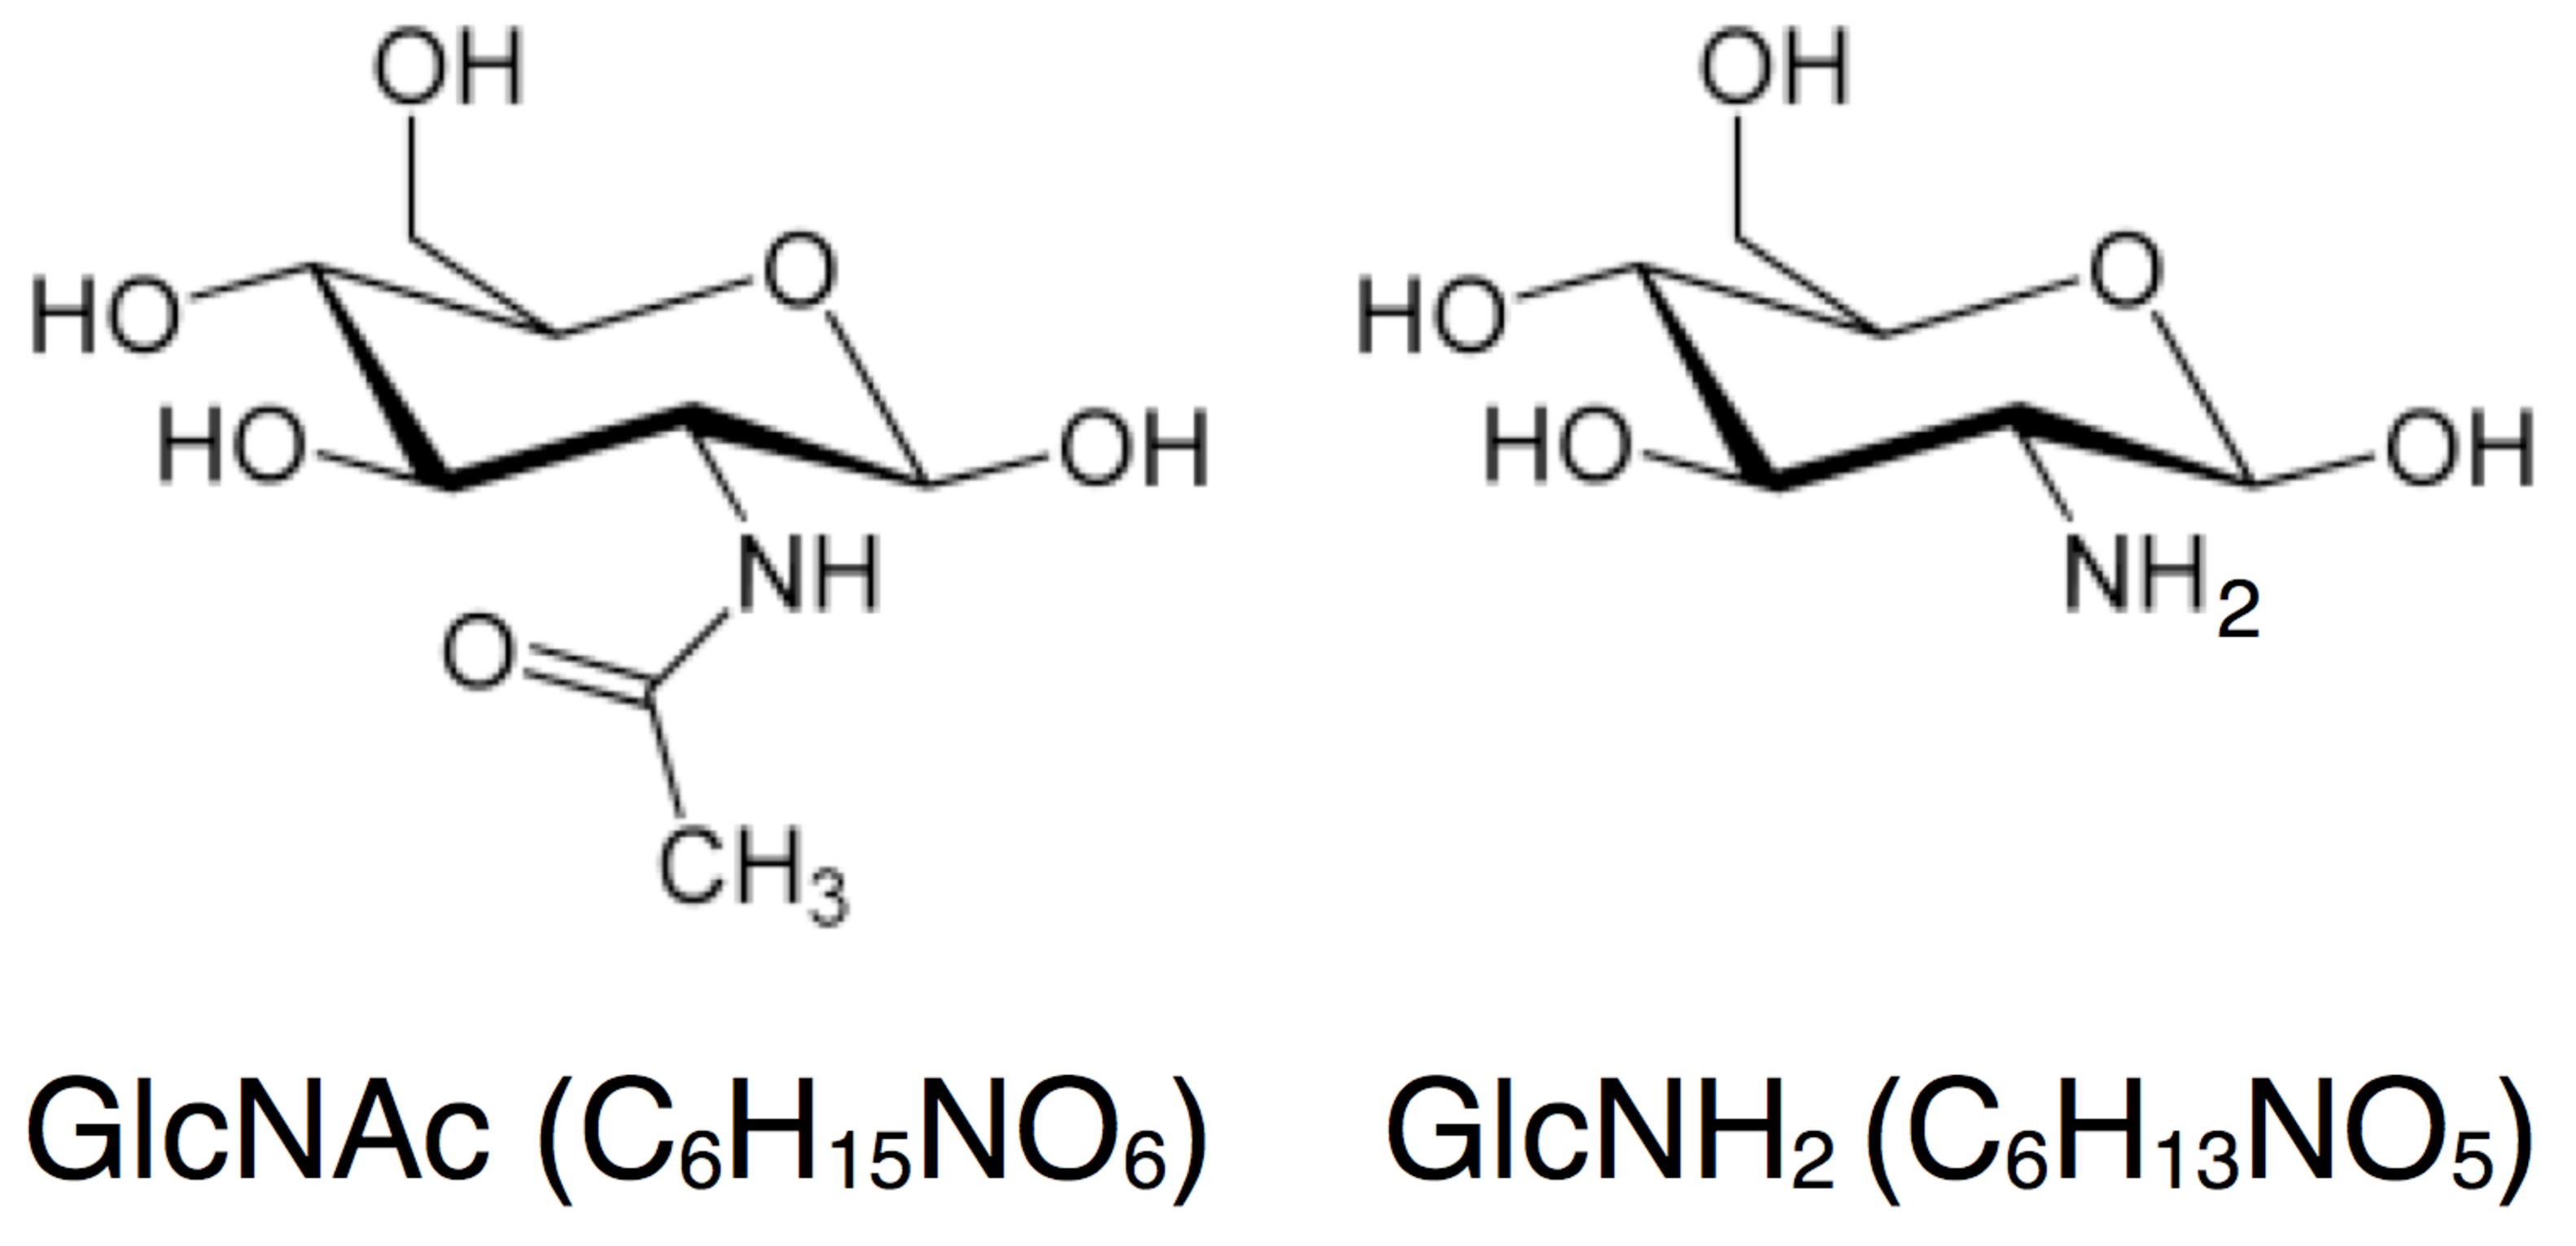
\includegraphics[width=4in]{figures/results4/sugar_structures.pdf}
\caption[Molecular structures of GlcNAc and GlcNH$_2$]{Molecular structures of $\beta$-N-acetyl-glucosamine (GlcNAc) and $\beta$-glucosamine (GlcNH$_2$).}
\label{fig:nag}
\end{figure}

\begin{figure}[htbp]
\centering
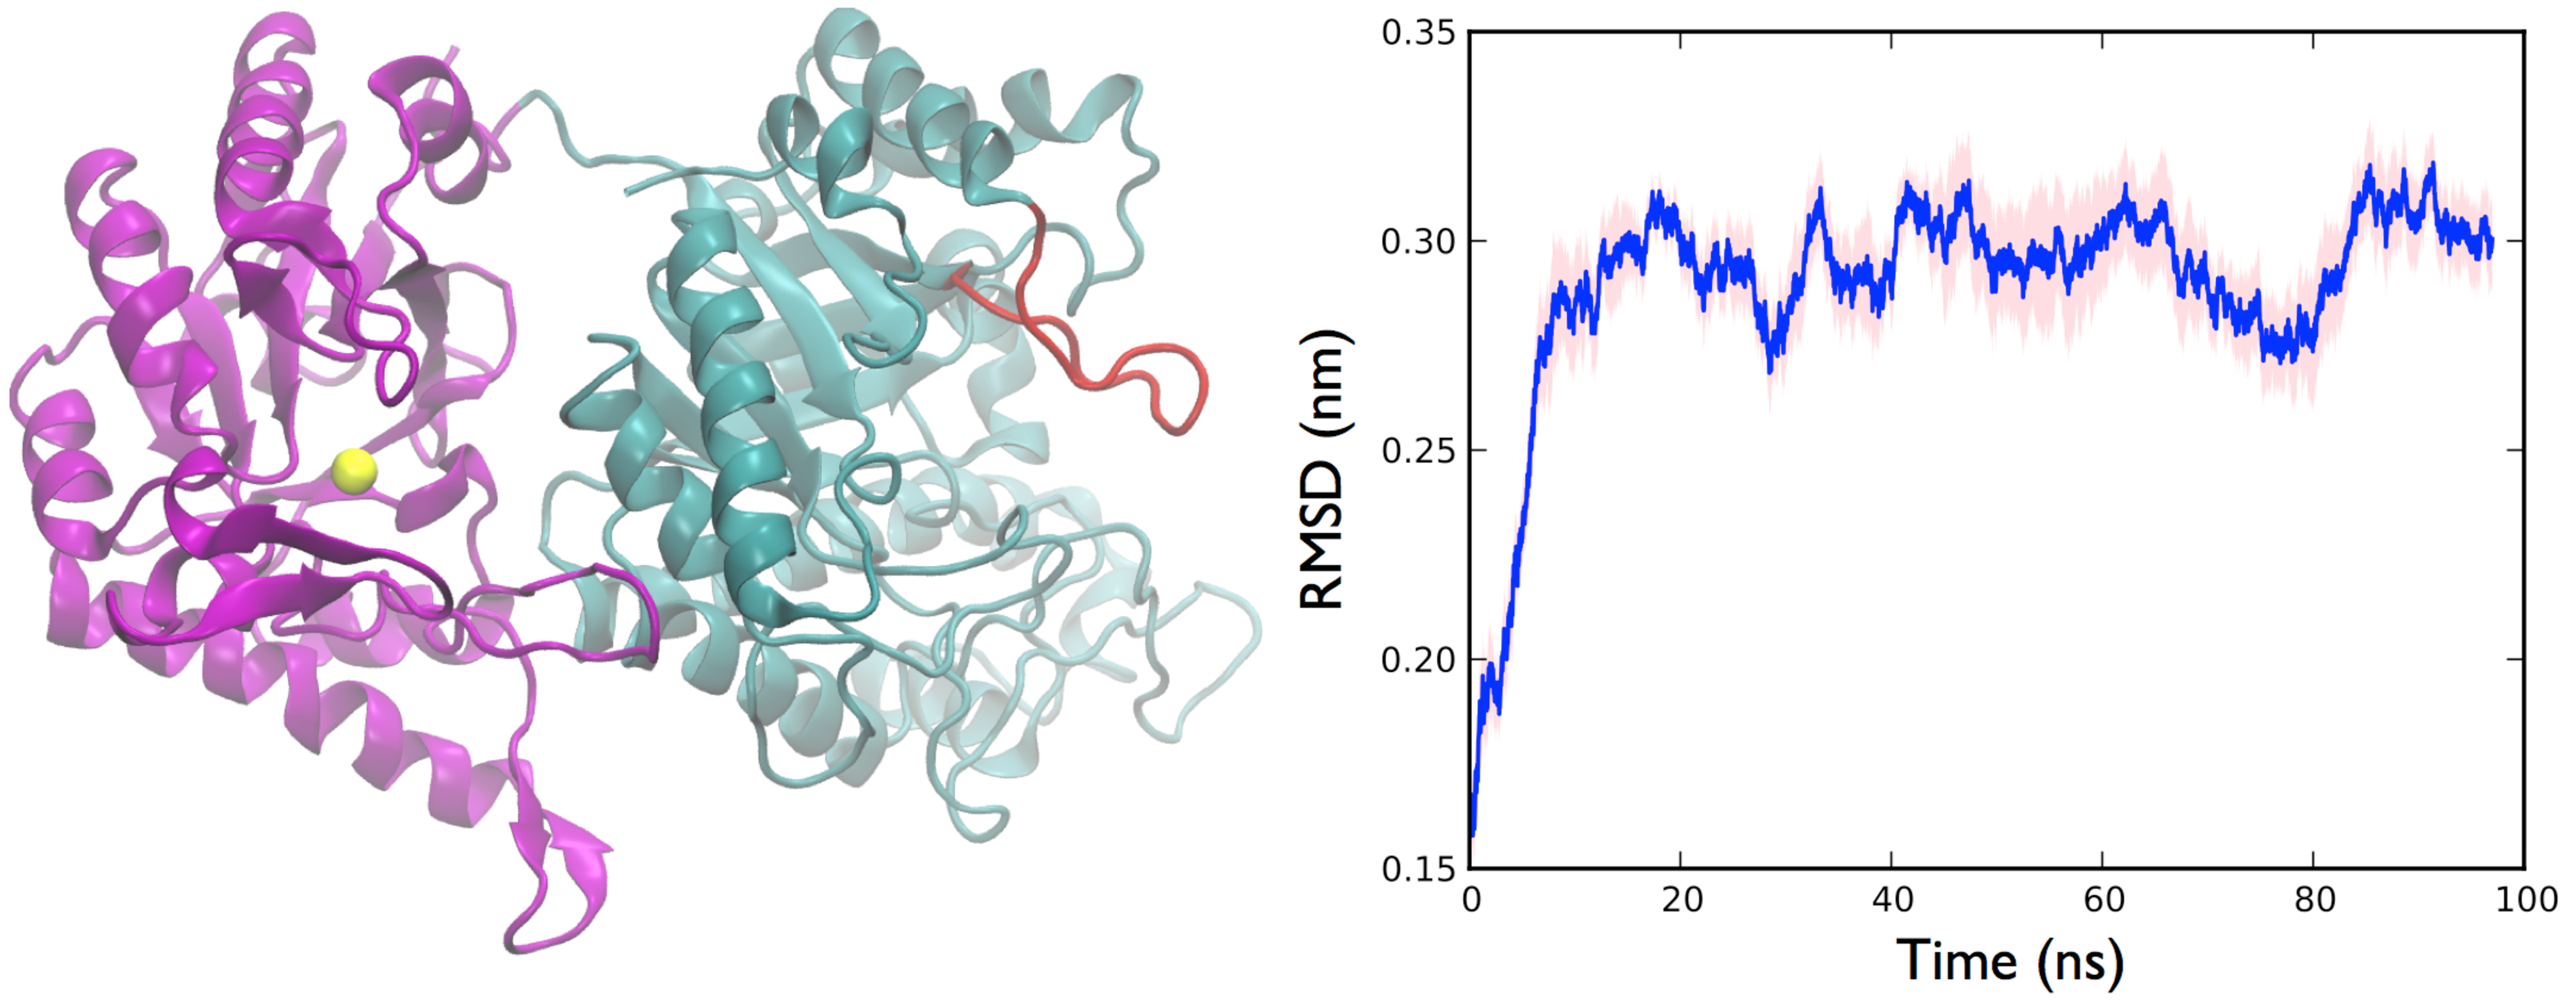
\includegraphics[width=6in]{figures/results4/protein_only.pdf}
\caption[Structure of PgaB and RMSD vs. time]{(A) Cartoon representation of the structure of chimeric PgaB. The N-terminal and C-terminal domain is represented in Magenta and Cyan, respectively.  Ni(II)+ is shown in a ball representation in yellow. The residues 610-623 in the flexible loop region which caps the groove in the C-terminal domain is represented in red. (B) Average RMSD of the protein from the crystal structure, in the presence of GlcNAc, with the loop region spanning residues 610-623 removed. Error in the mean is represented by the pink shaded region.}
\label{fig:rmsd}
\end{figure}

\begin{figure}[htbp]
\centering
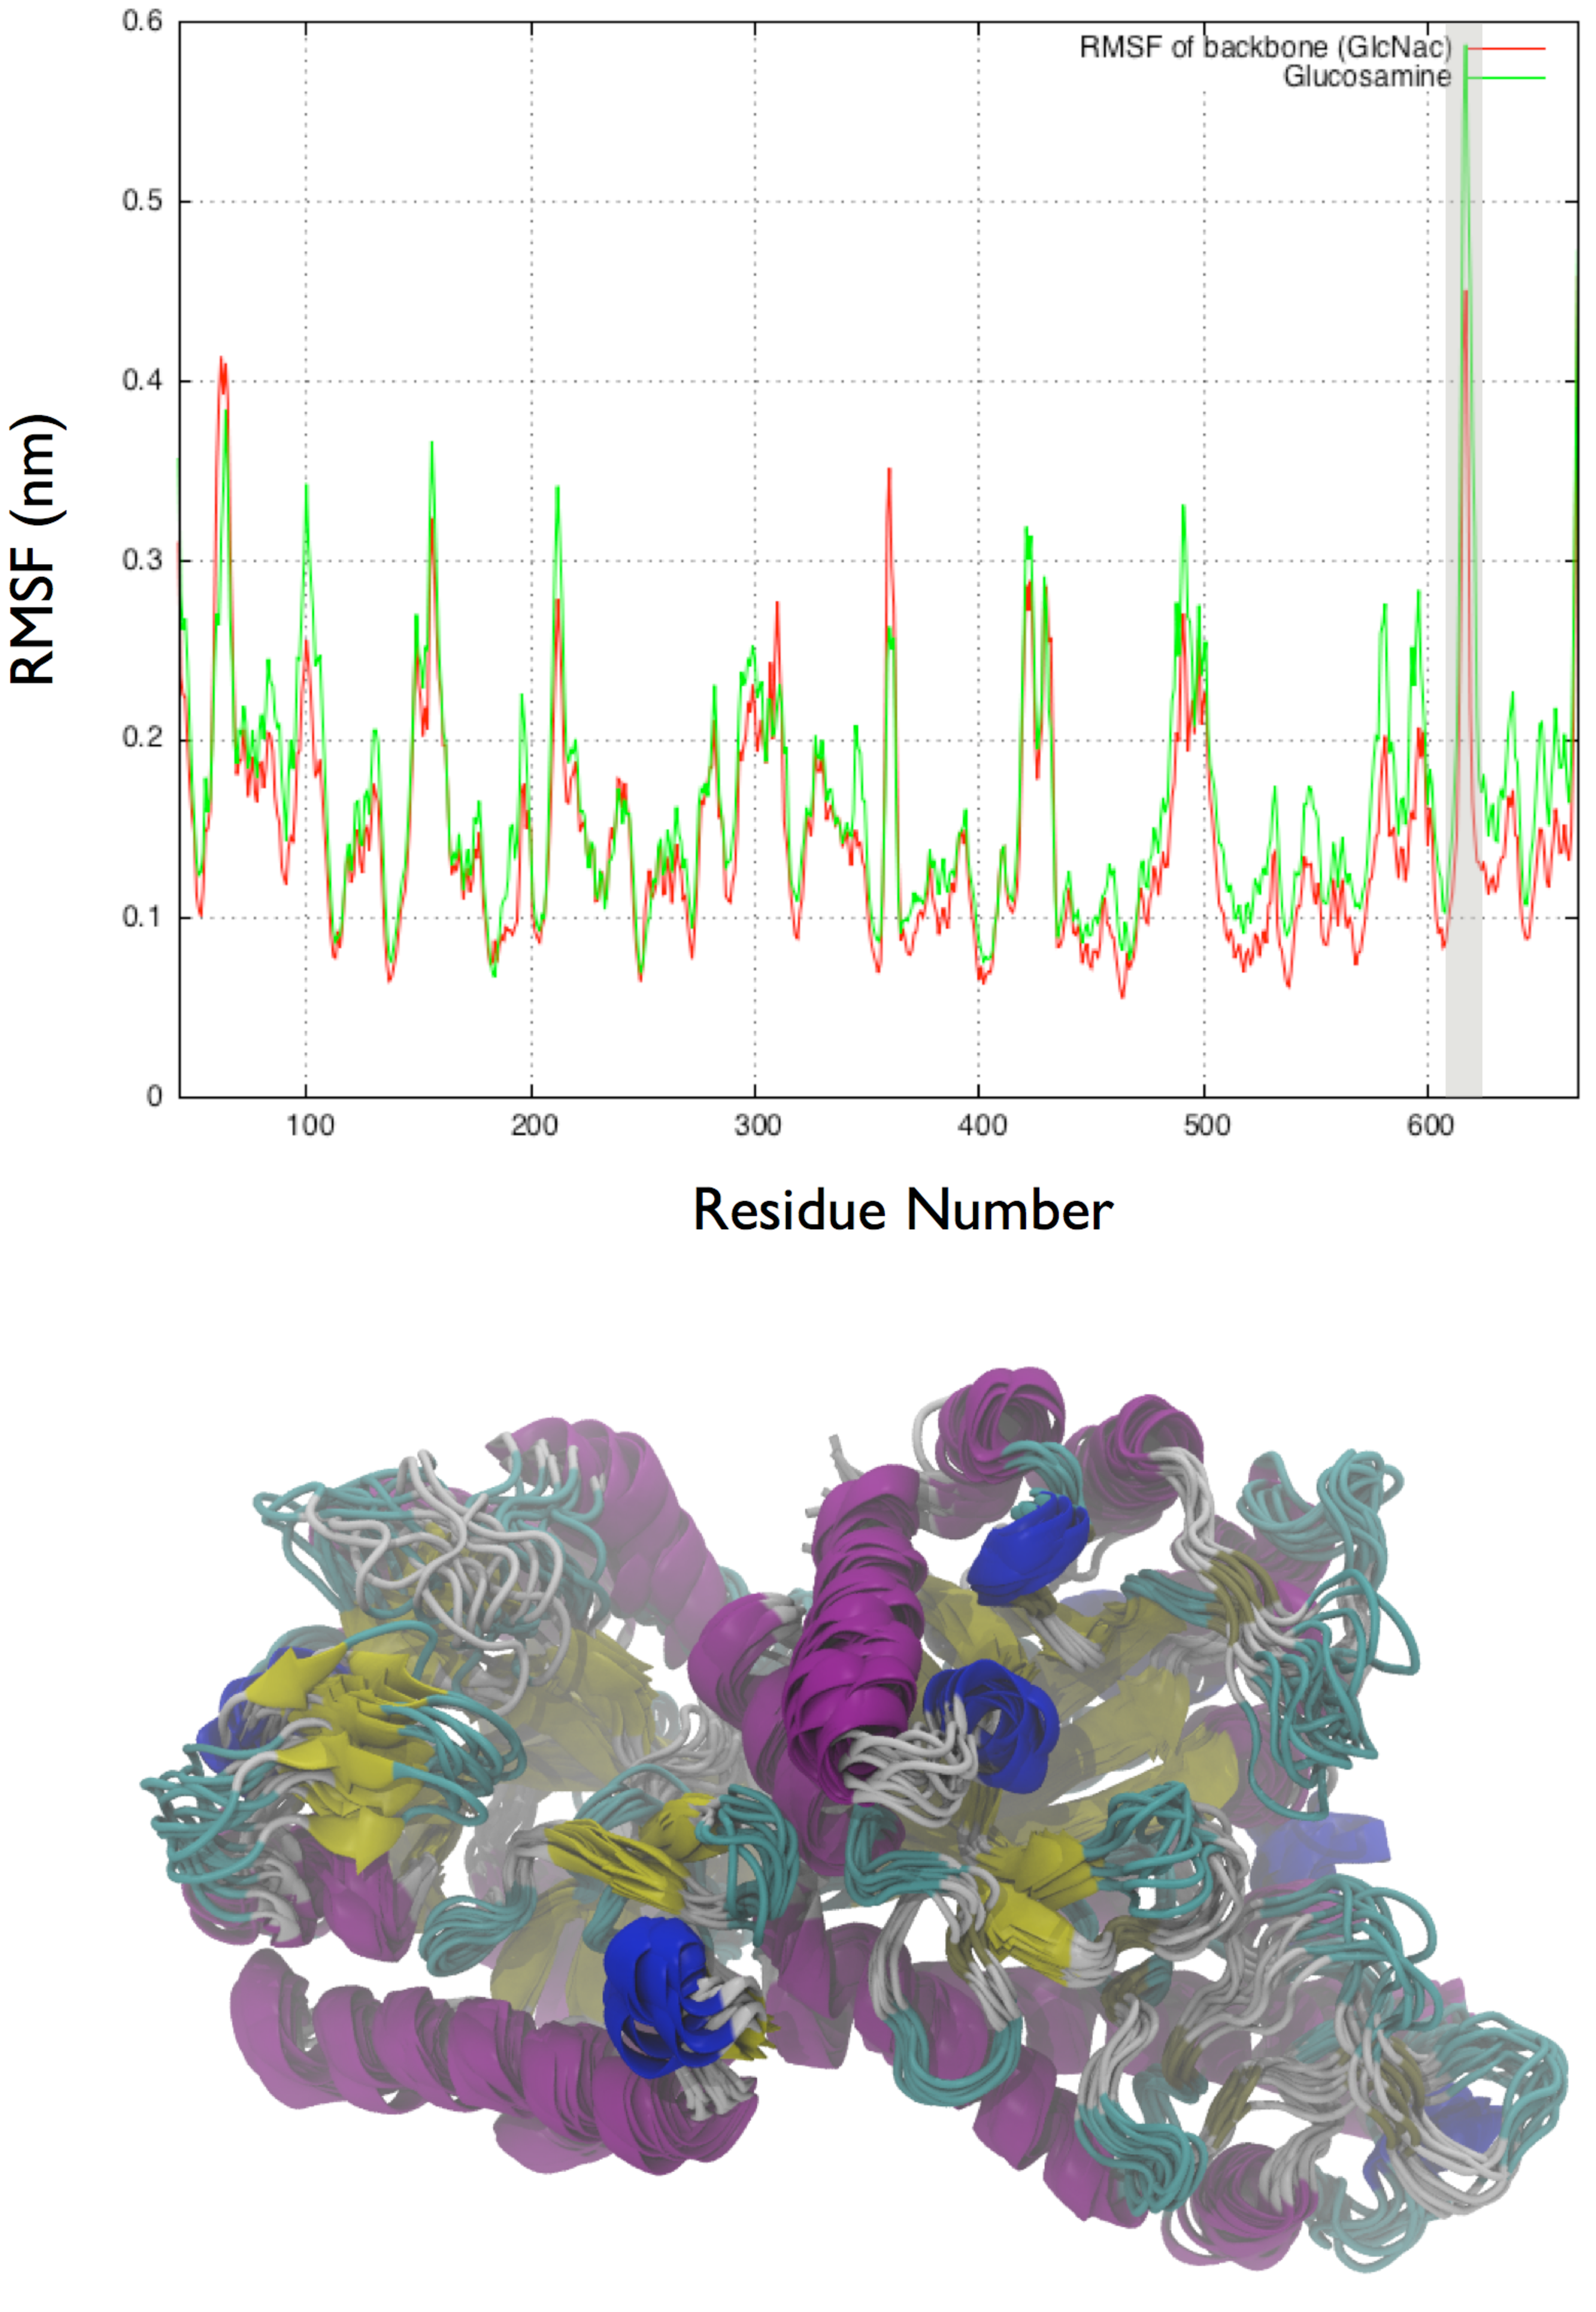
\includegraphics[width=4in]{figures/results4/rmsf.pdf}
\caption[RMSF of residues in PgaB]{Average root-mean-square fluctuation of residues in PgaB in the presence of (A) GlcNAc and (B) Glucosamine.}
\label{fig:rmsf}
\end{figure}

\begin{figure}[htbp]
\centering
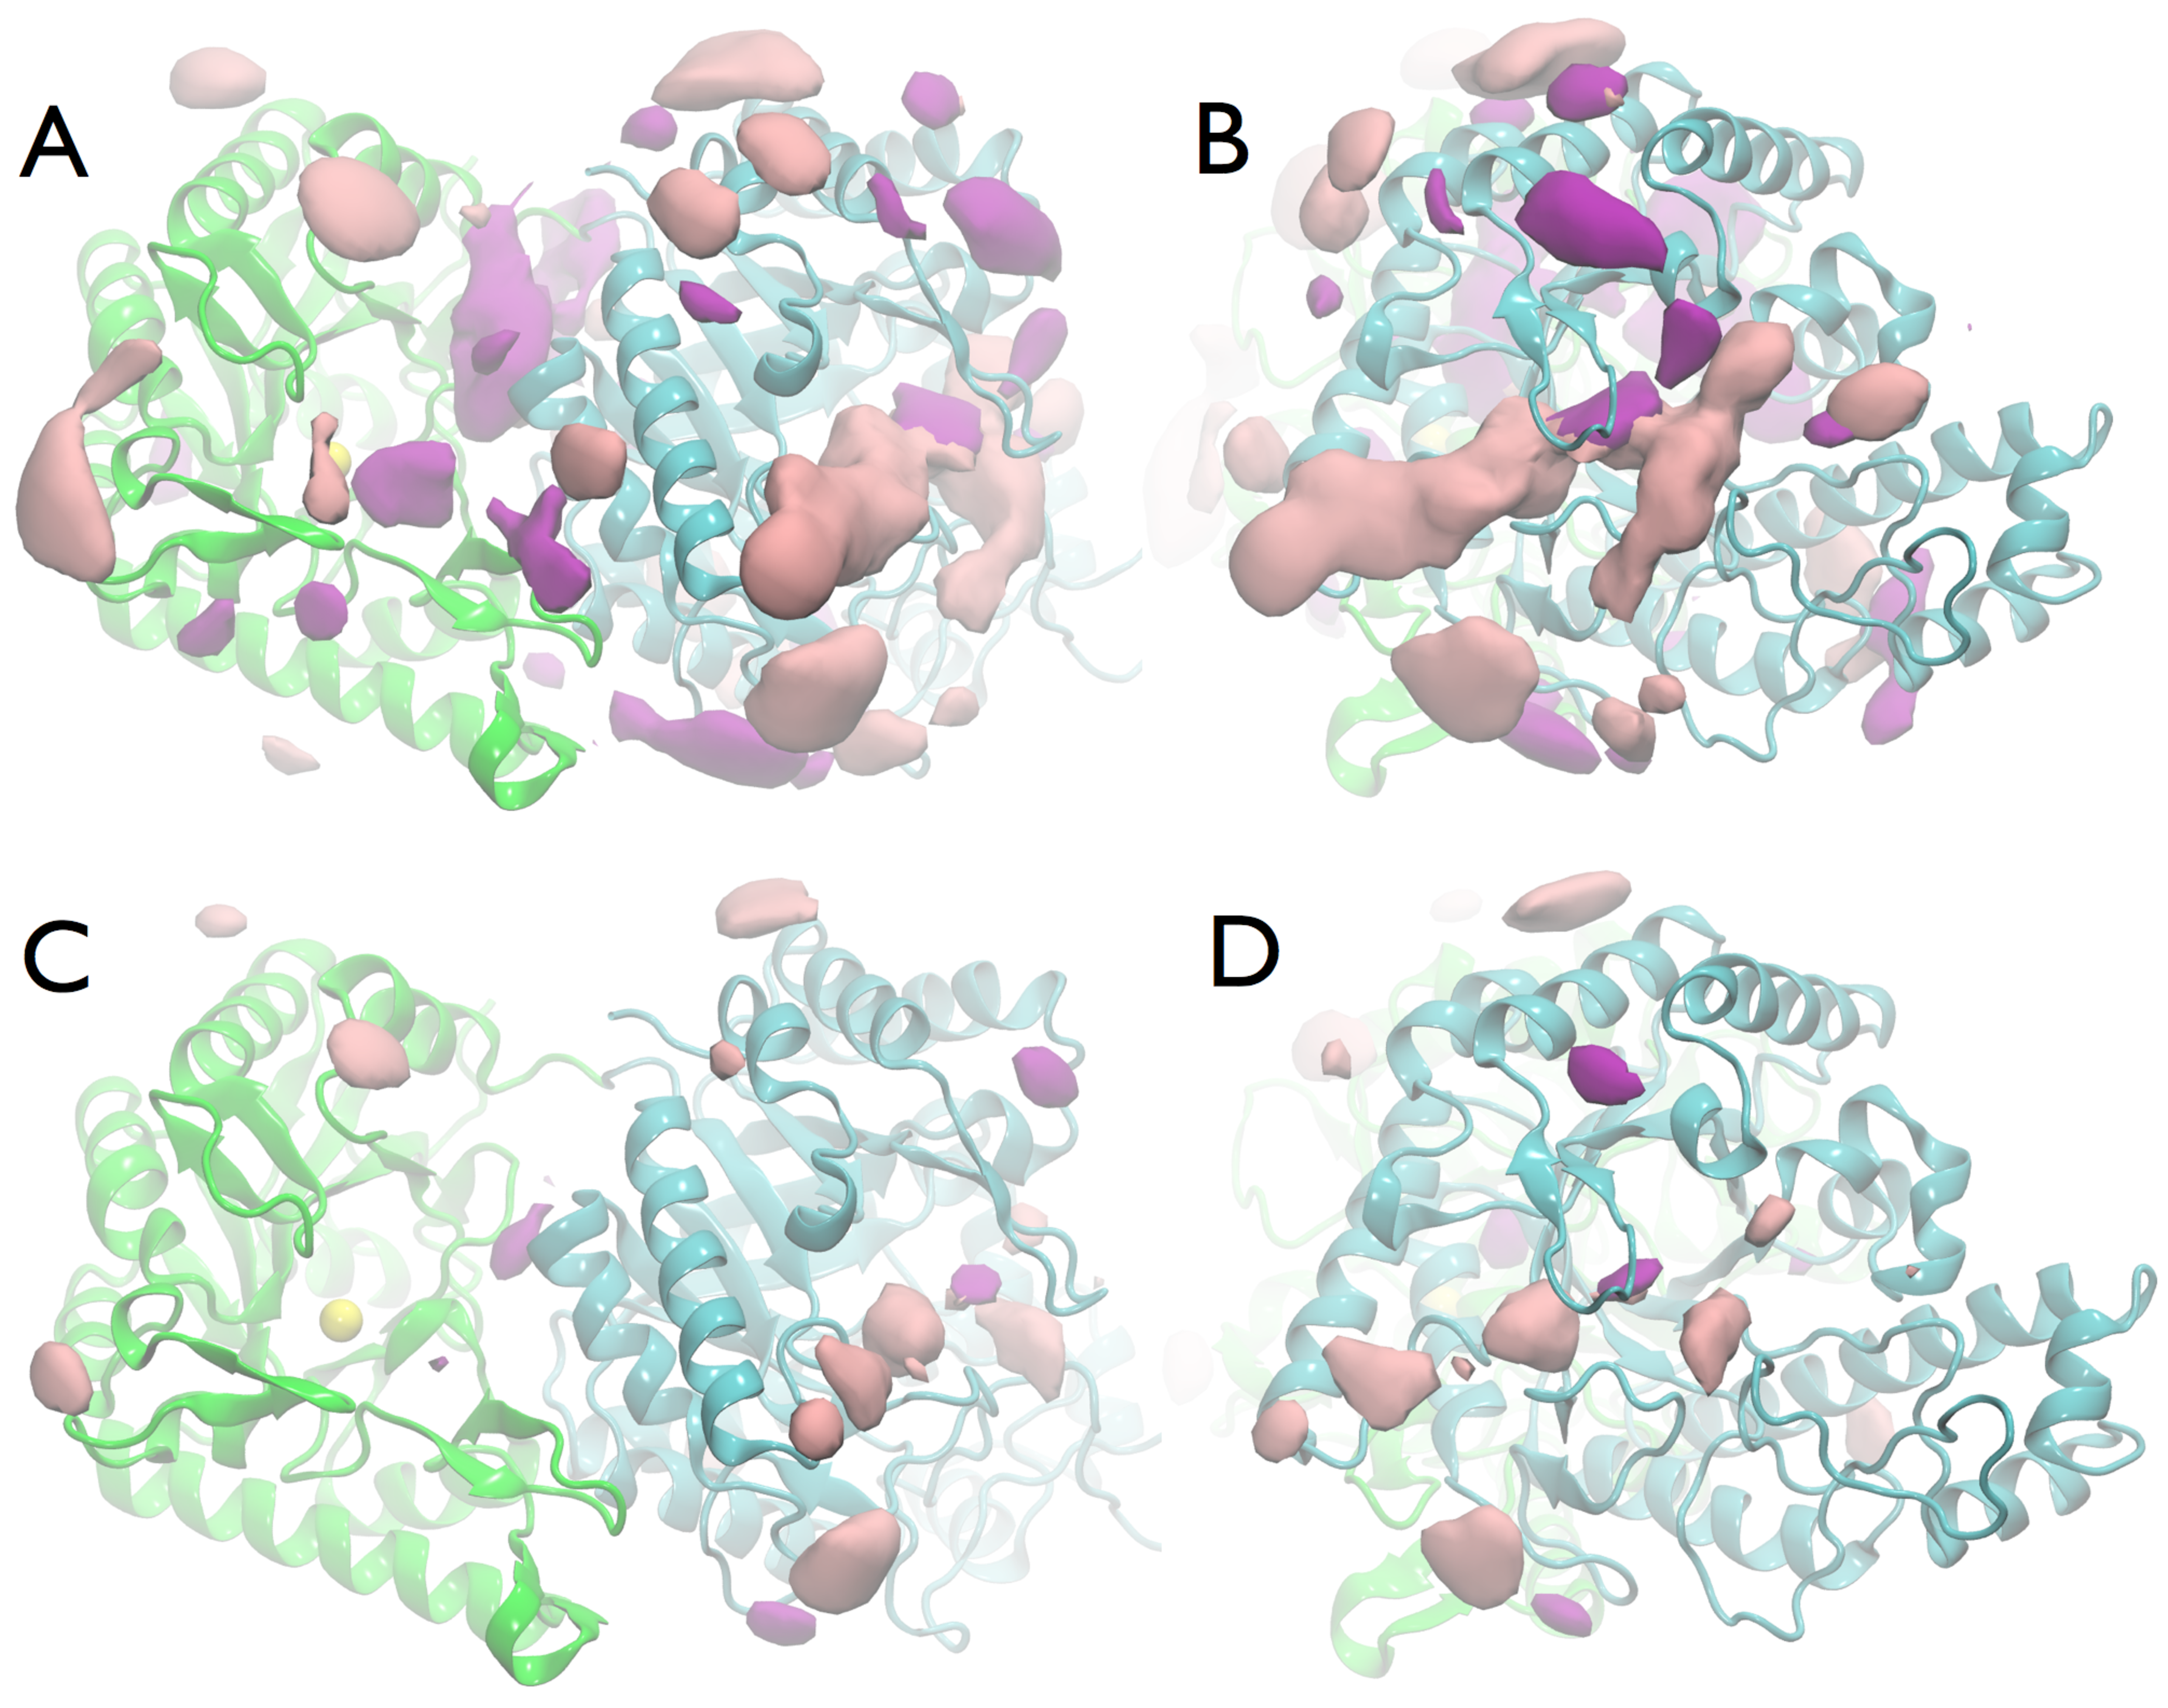
\includegraphics[width=6.25in]{figures/results4/glcnac_glucosamine_merged_sdf.pdf}
\caption[Spatial probability densities of bound GlcNAc (purple) and \glucosamine]{Spatial probability densities of bound GlcNAc (purple) and \glucosamine\ (pink). Binding densities overlapped with a cartoon representation of the energy minimized crystal structure of PgaB. The protein is shown facing the active site in (A) and (C), and shown facing the C-terminal domain in (B) and (D). In each view, binding densities are depicted at occupancies of 0.15 in (A)-(B), and 0.25 in (C) - (D). In our coloring scheme, residue numbers 43 to 310 and numbers 311 to 667 represent N- (green) and C-terminal (cyan) domains, respectively.}
% Note that the magenta colored densities over PgaB-NT cover conserved residues in CE4. (These residues are highlighted in magenta in Little et. al. in Figure S1. ) \textbf{Id the residues and list them in the text and in the caption. Need to add the isovalues for the top and bottom two panels.}
\label{fig:sdf}
\end{figure}

\begin{figure}[htbp]
\centering
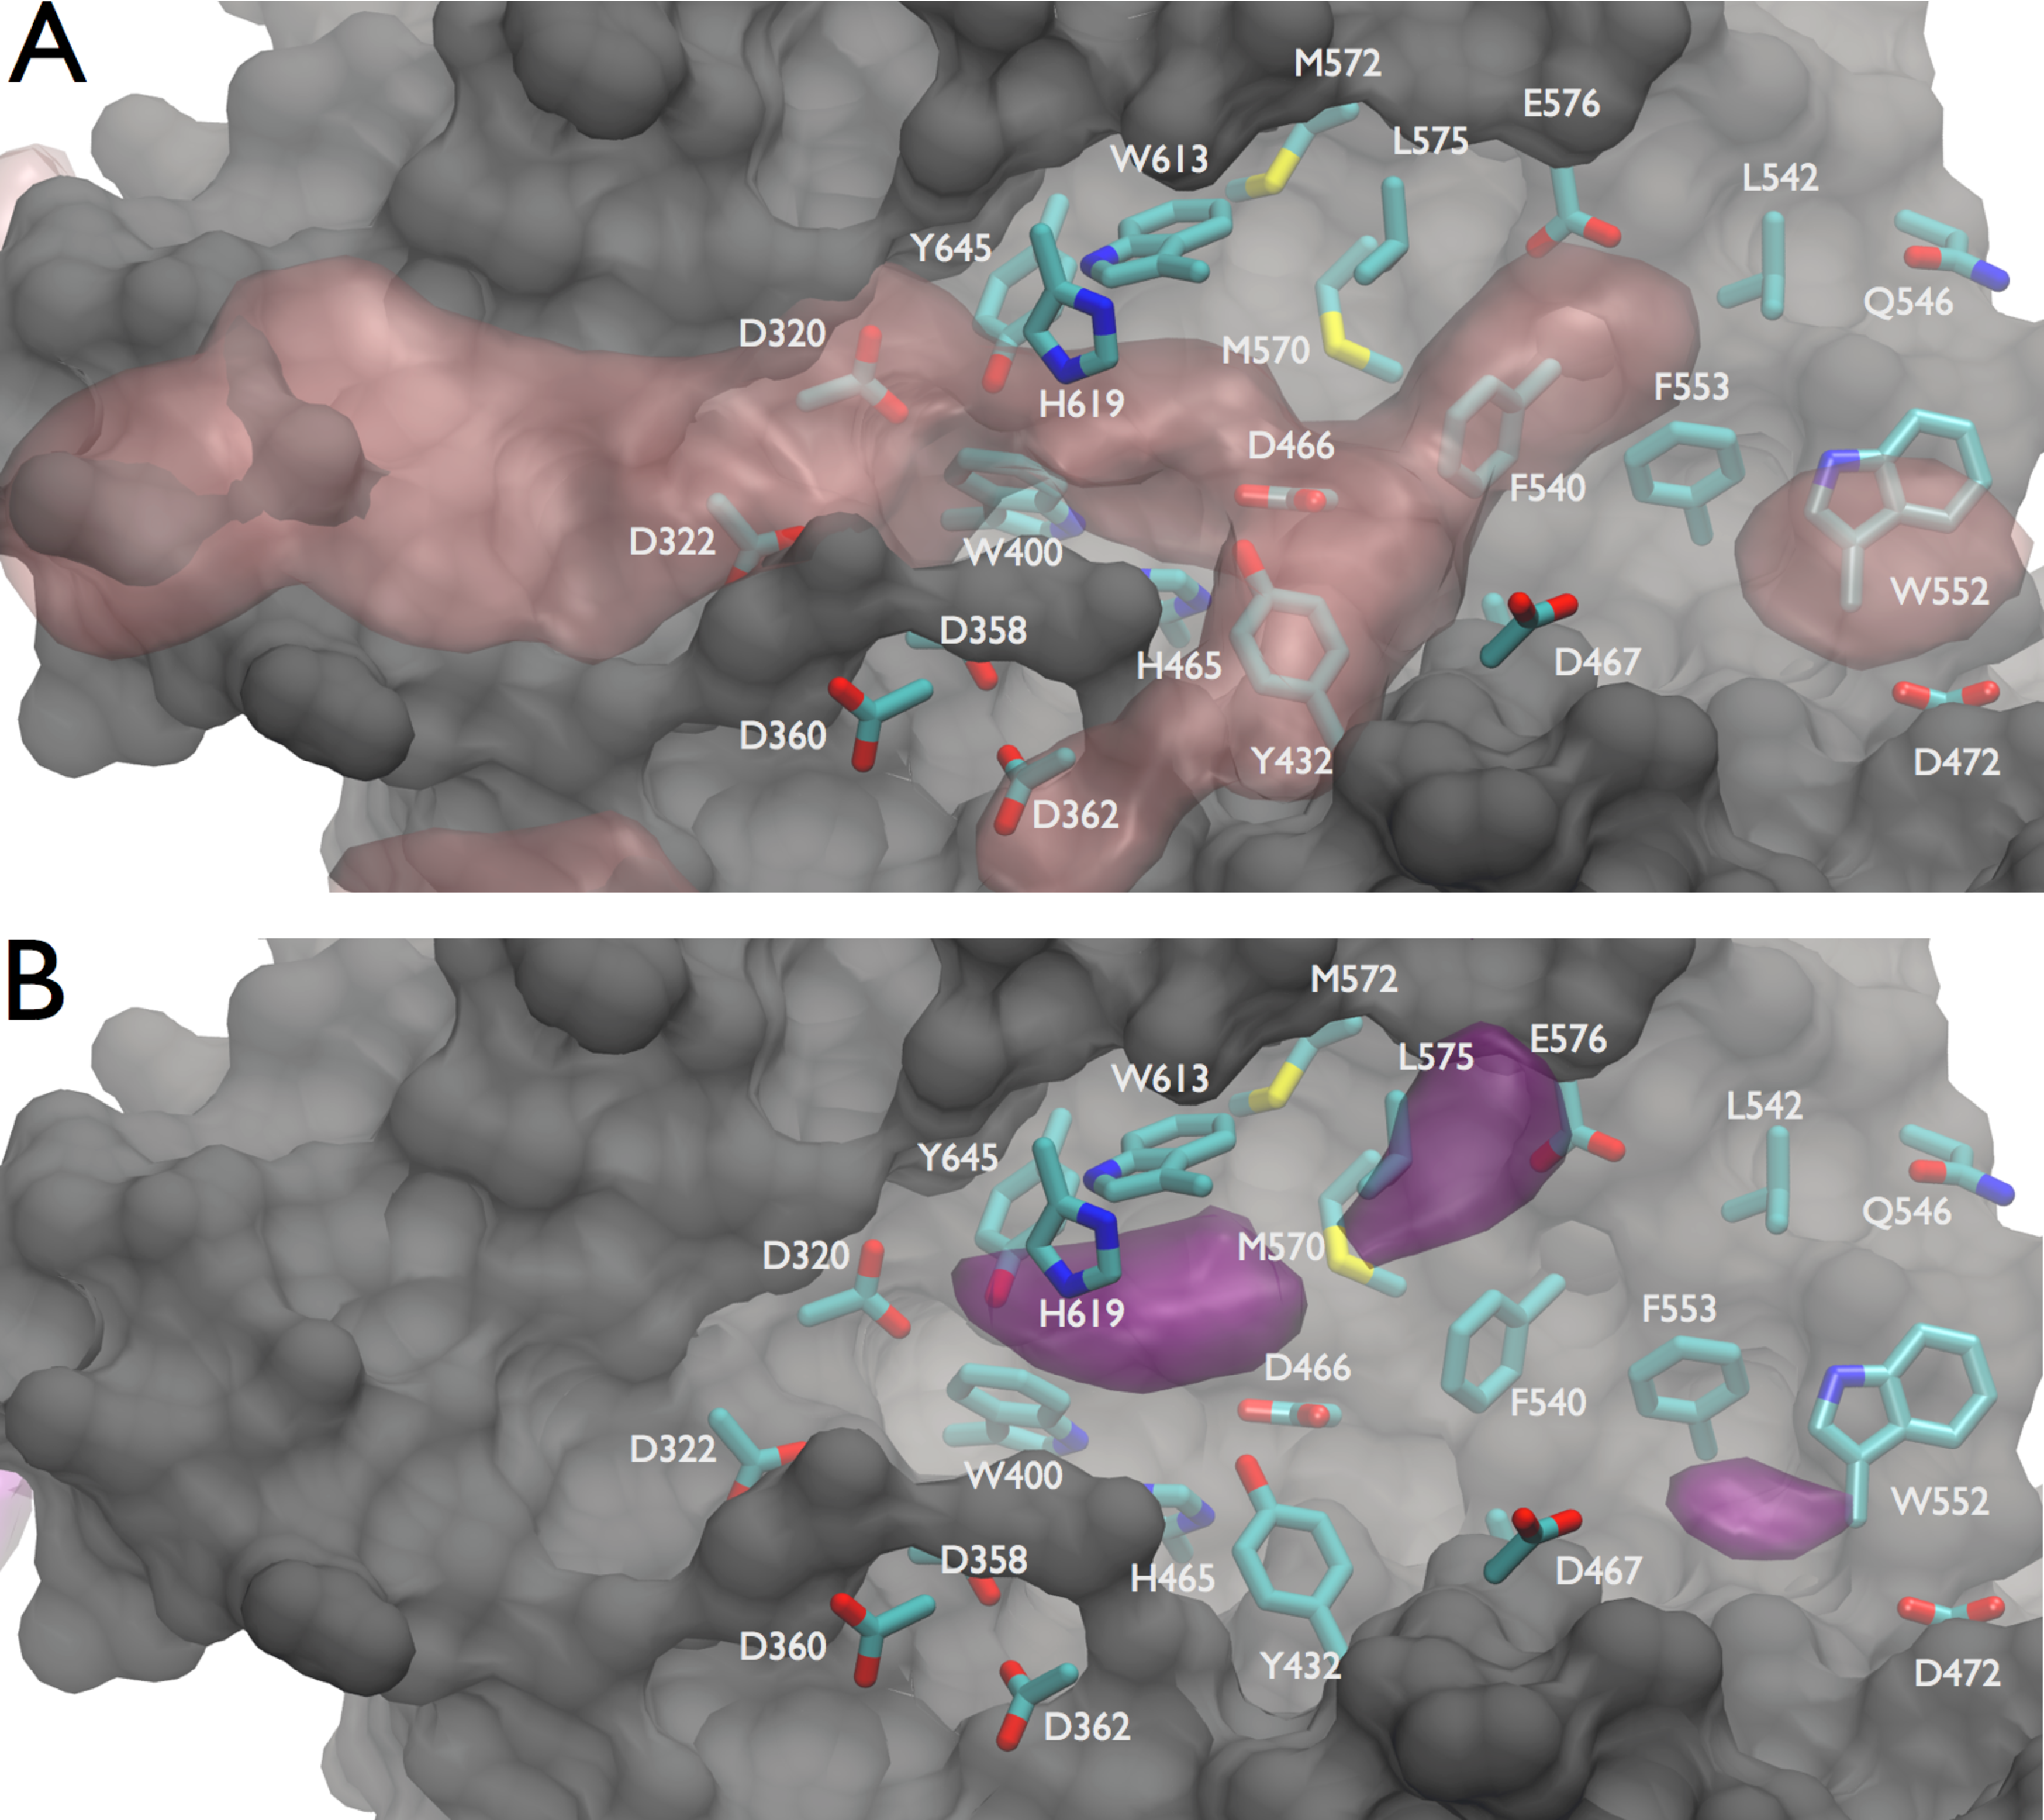
\includegraphics[width=6.25in]{figures/results4/cterm_groove_surf3.pdf}
\caption[Spatial probability densities of GlcNAc and GlcNH3+ in the C-terminal groove]{Spatial probability distribution shown at an occupancy of 0.15 for (A) \glucosamine\ and (B) GlcNAc in the binding groove of the C-terminal domain. The residues in the groove are shown in stick representations.}
\label{fig:groove}
\end{figure}

\begin{figure}[htbp]
\centering
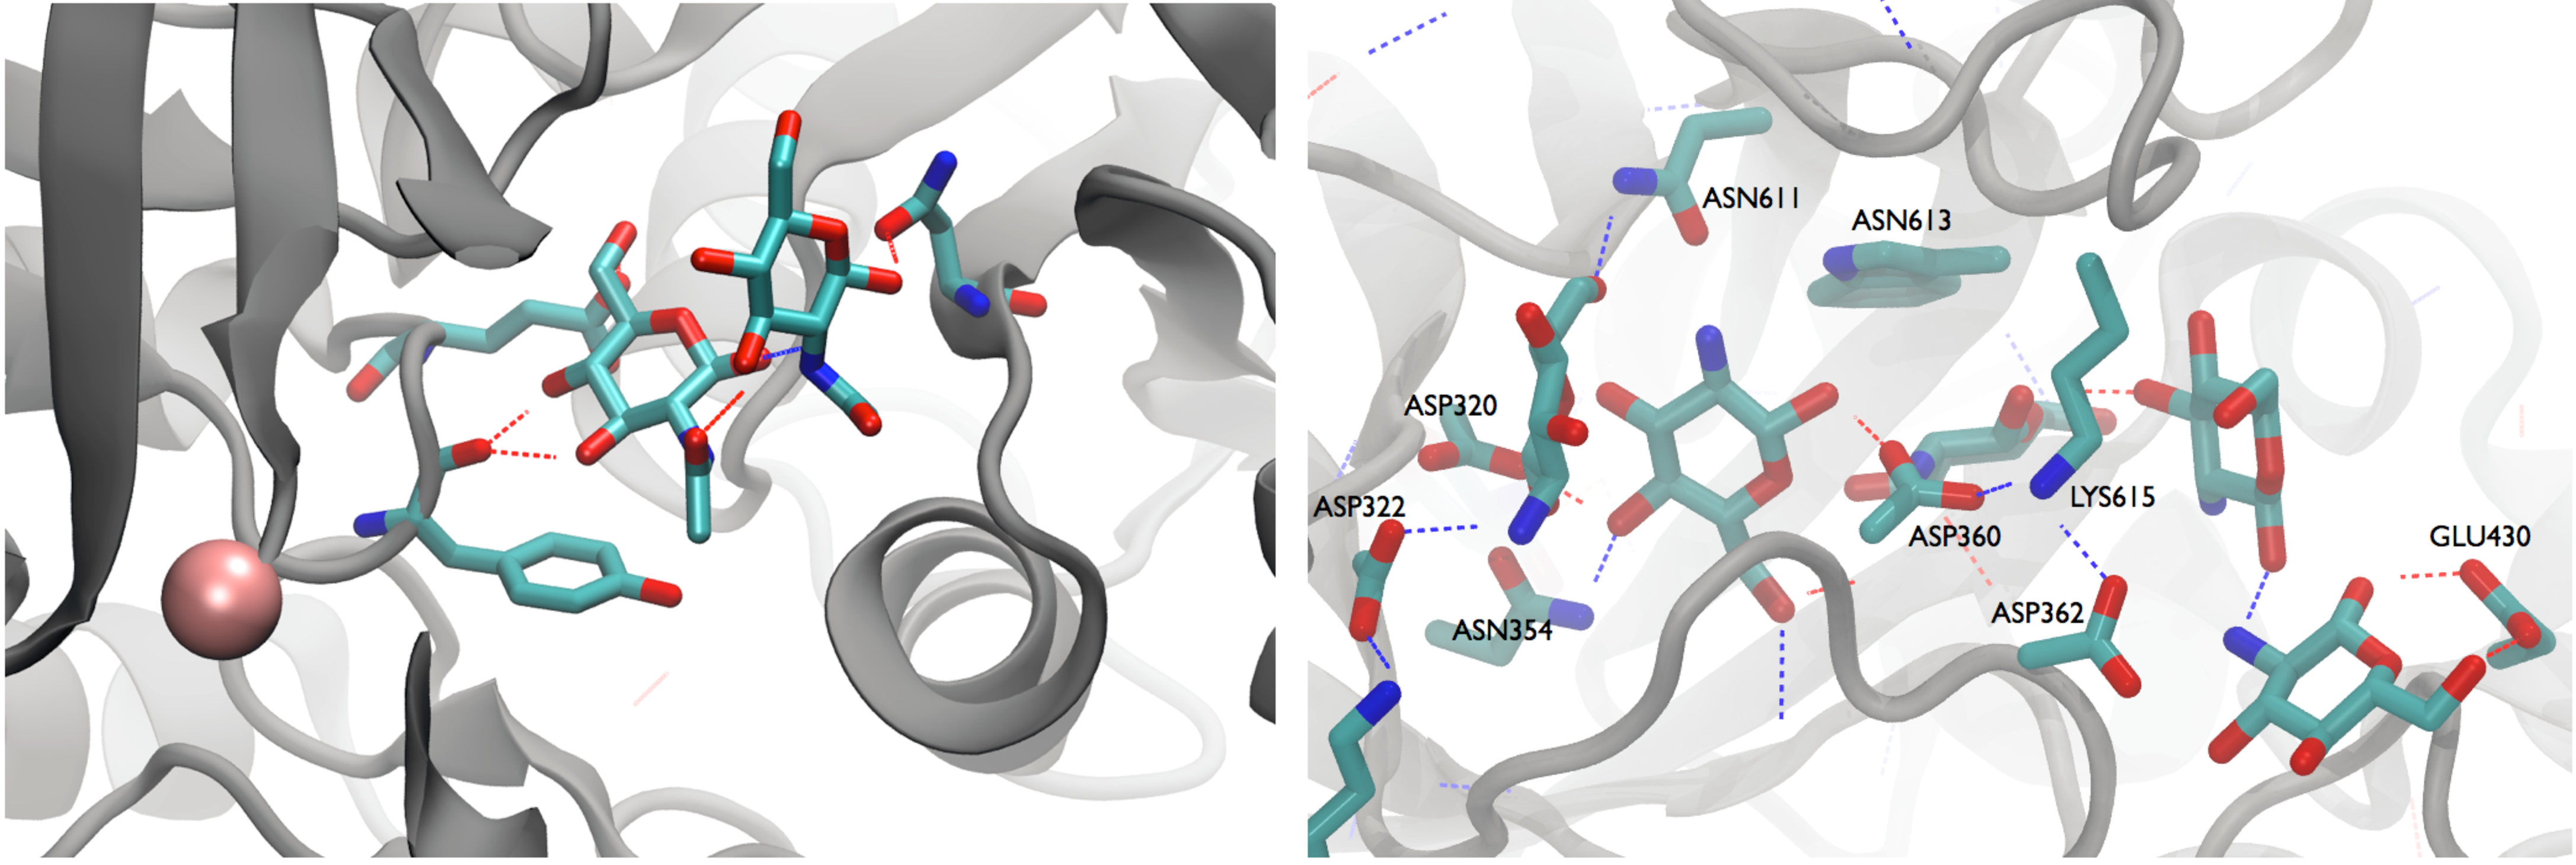
\includegraphics[width=6.25in]{figures/results4/binding_modes.pdf}
\caption[Example of glucosamine molecules binding in the C-terminal groove] {Example binding modes of glucosamine in the C-terminal groove. \glucosamine\ molecules bind in the C-terminal domain carbohydrate-binding groove by forming intermolecular hydrogen bonds with polar and charged residues and forming nonpolar contacts by stacking face-to-face with aromatic moieties.}
\label{fig:glucosamine_binding_modes_c_term}
\end{figure}

\begin{figure}[htbp]
\centering
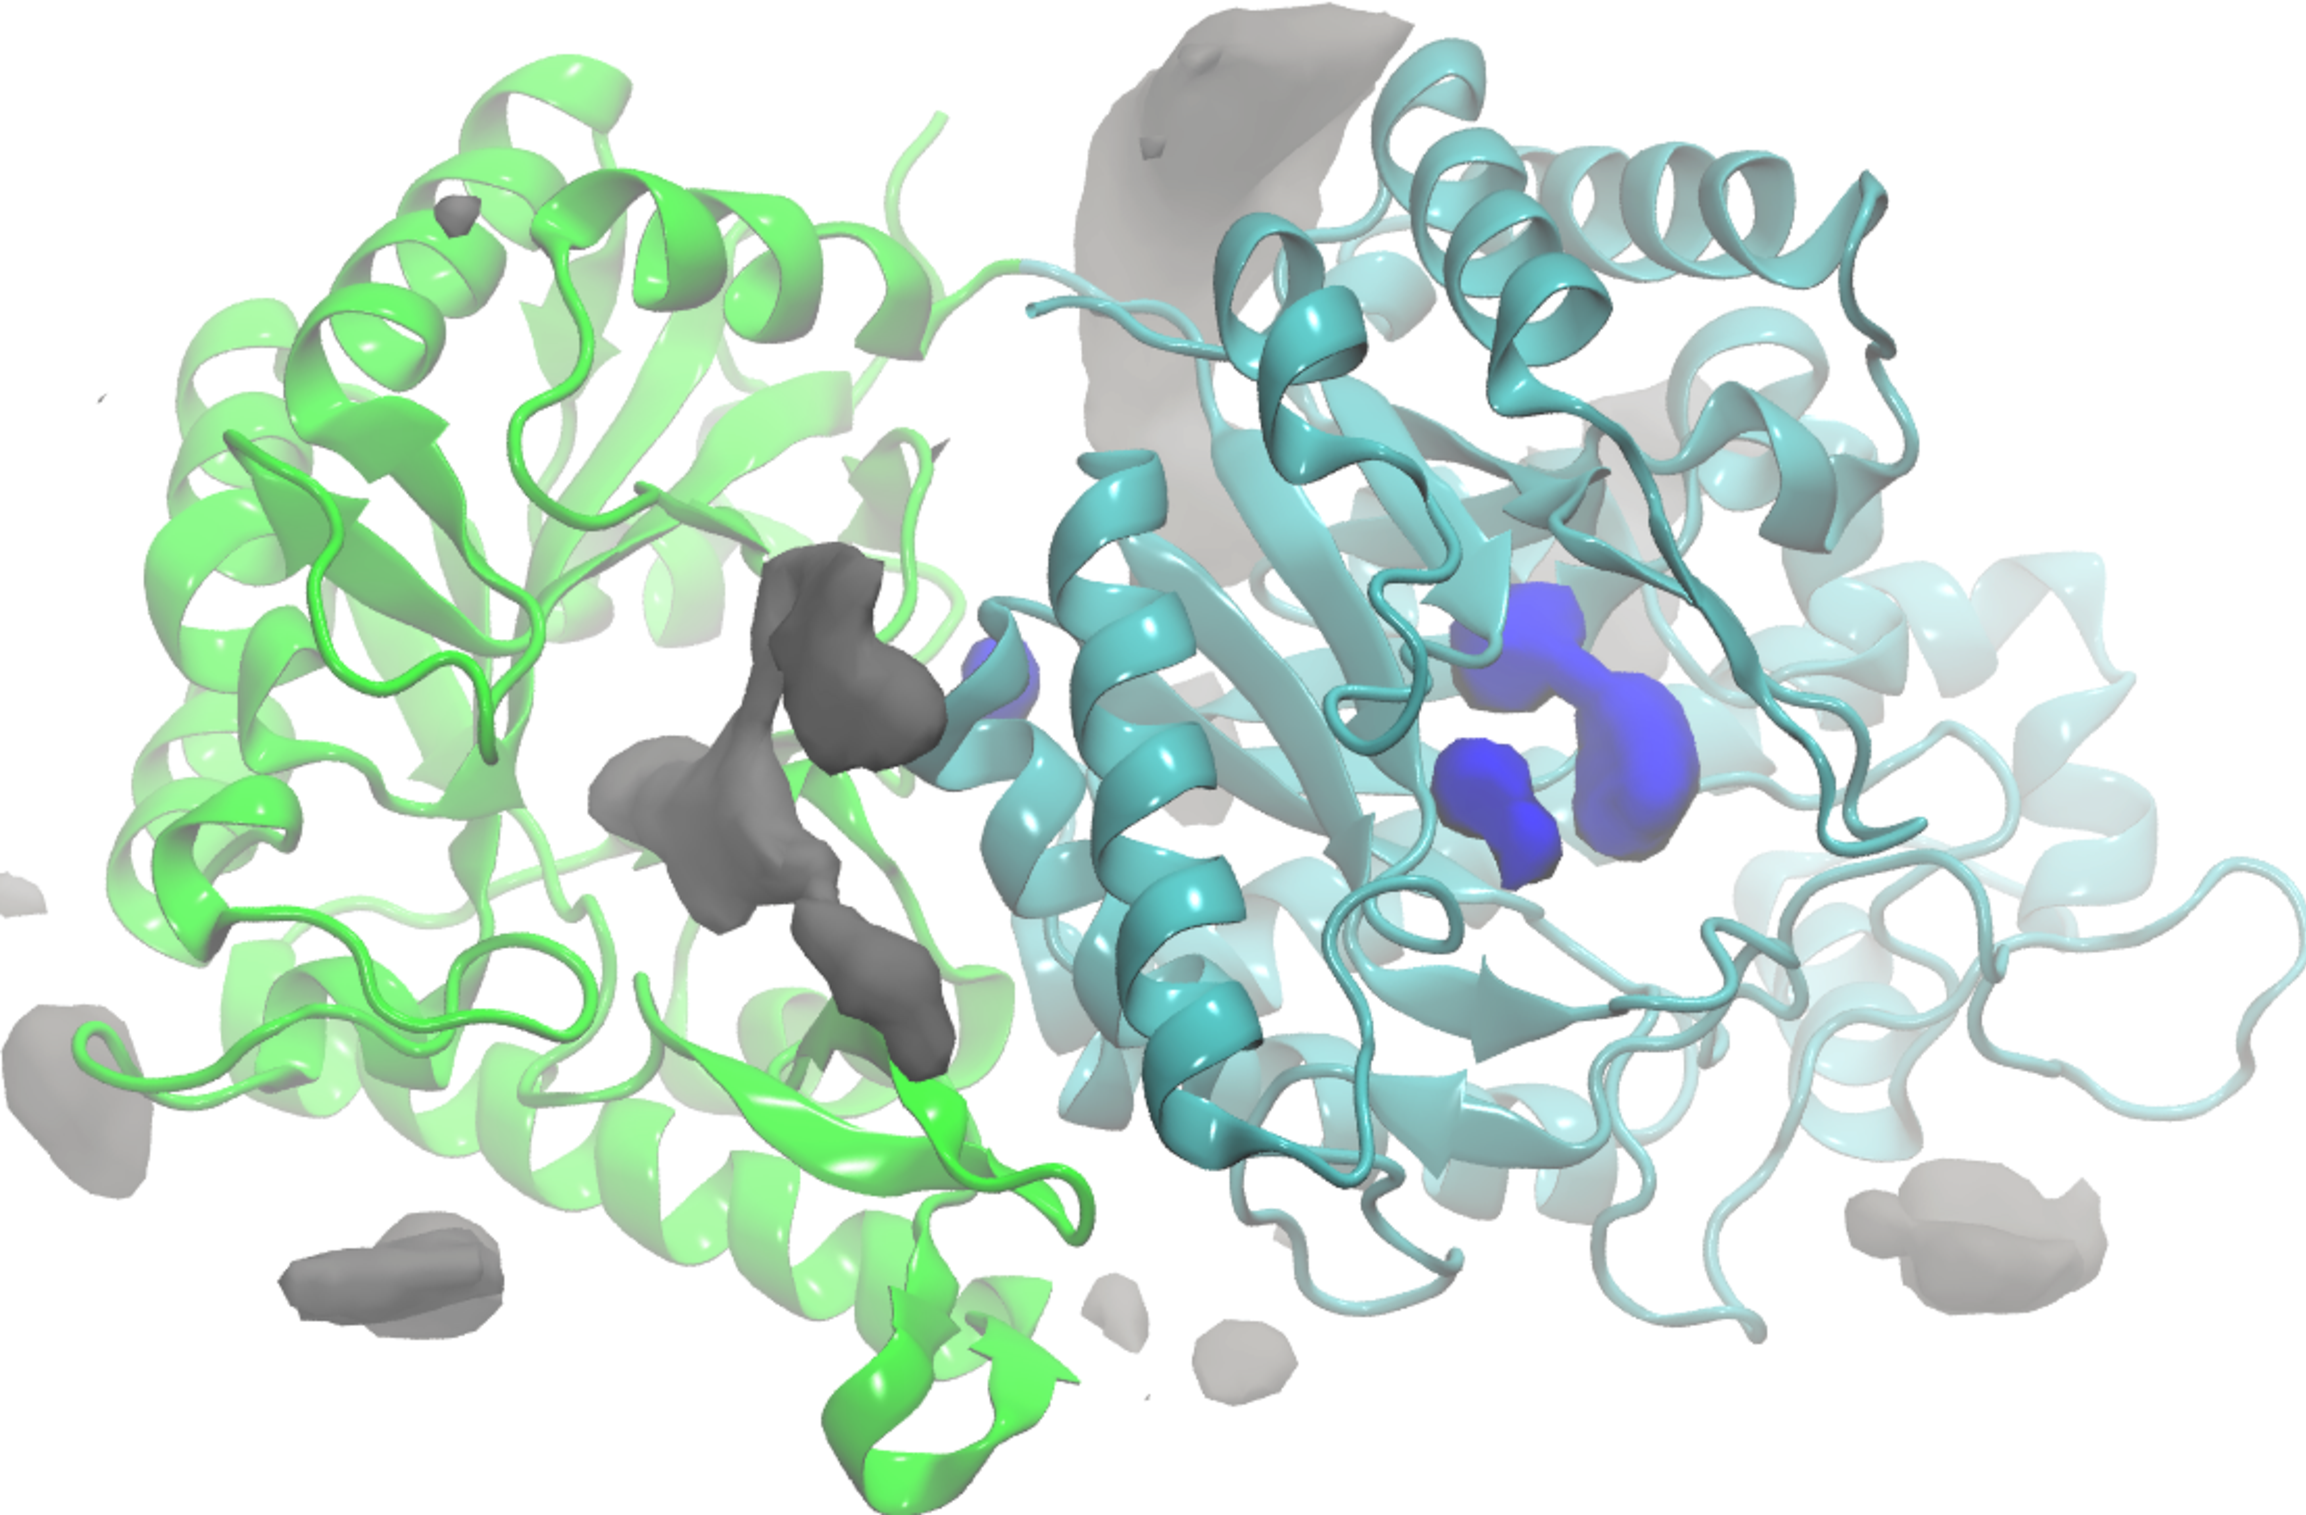
\includegraphics[width=6.25in]{figures/results4/pgab_glucosamine_salt_densities.pdf}
\caption[Ionic distribution]{Spatial probability distribution of sodium (blue) and chloride (grey) ions depicted at an isovalue of 0.005. The protein is depicted in a cartoon representation, with N- and C-terminal domains colored in green and cyan, respectively.}
\label{fig:salt_density_distribution}
\end{figure}

\begin{figure}[htbp]
\centering
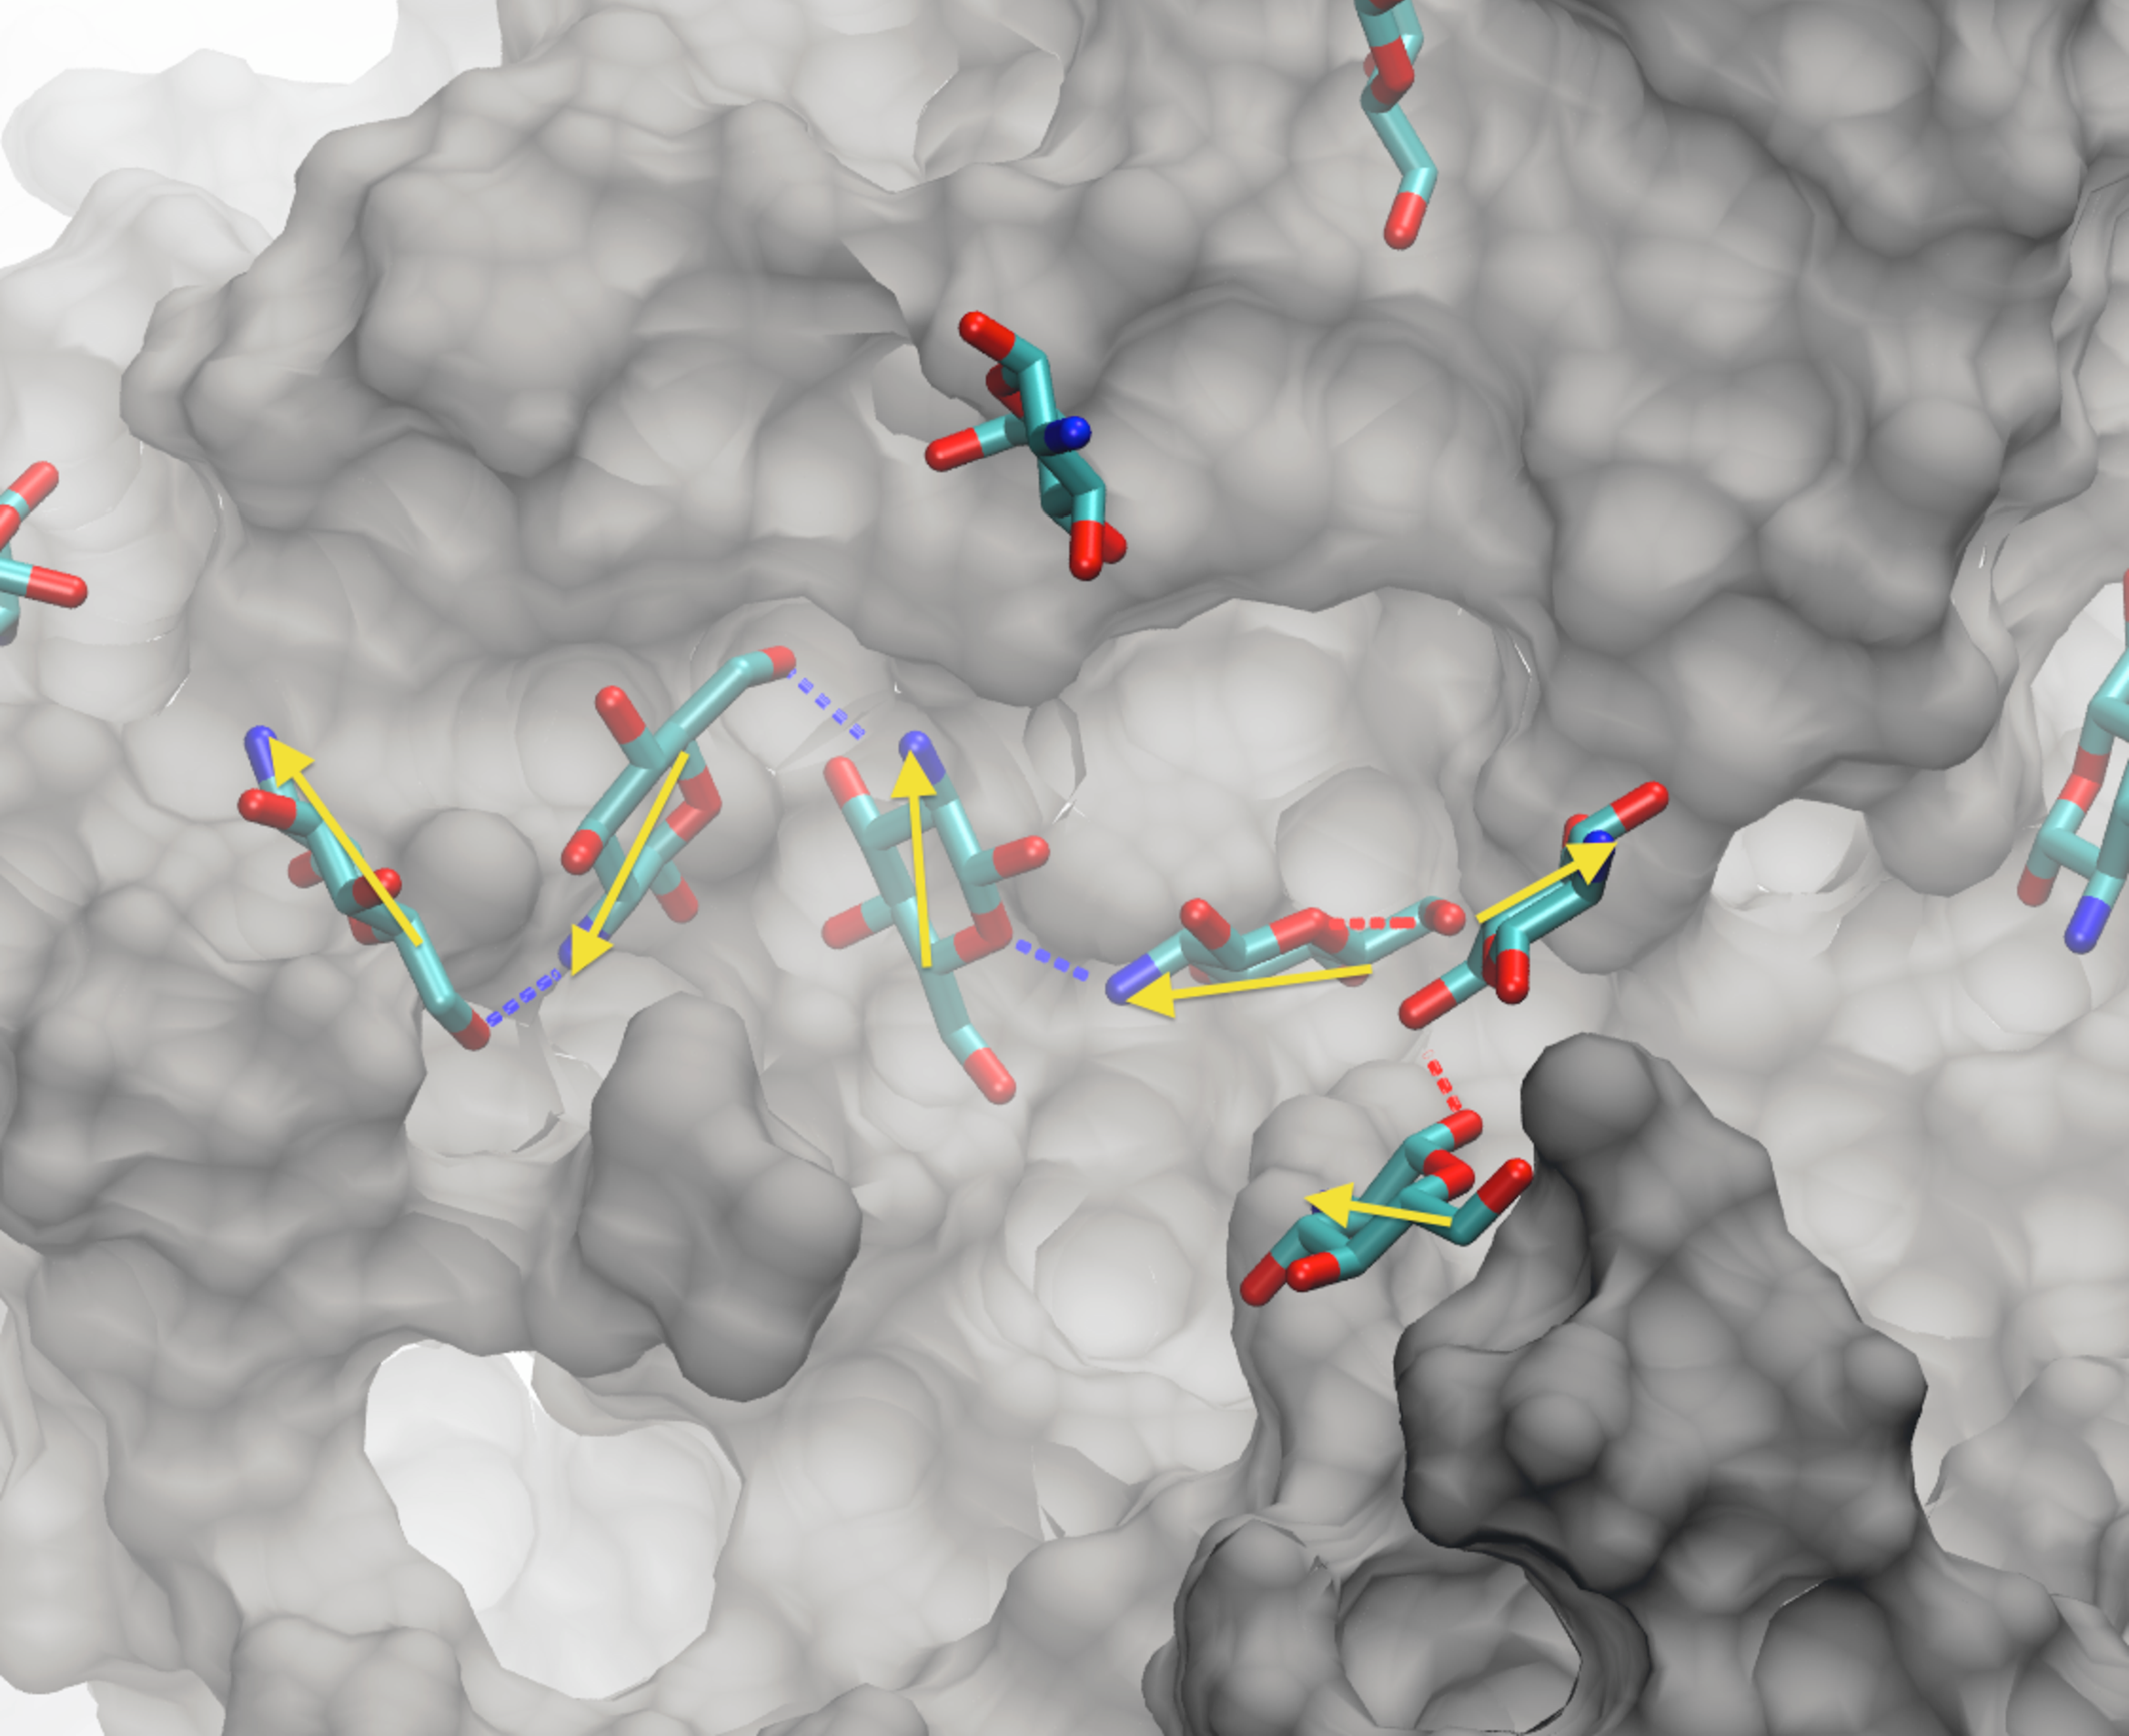
\includegraphics[width=6.25in]{figures/results4/glucosamine_binding_direction_suggestive.pdf}
\caption[Polymer directionality]{A linear chain of hydrogen-bonded \glucosamine\ molecules in the putative carbohydrate-binding groove of the C-terminal domain. The yellow arrows are drawn as a guide to highlight a putative chain directionality.}
\label{fig:directionality}
\end{figure}

%\begin{figure}[htbp]
%\centering
%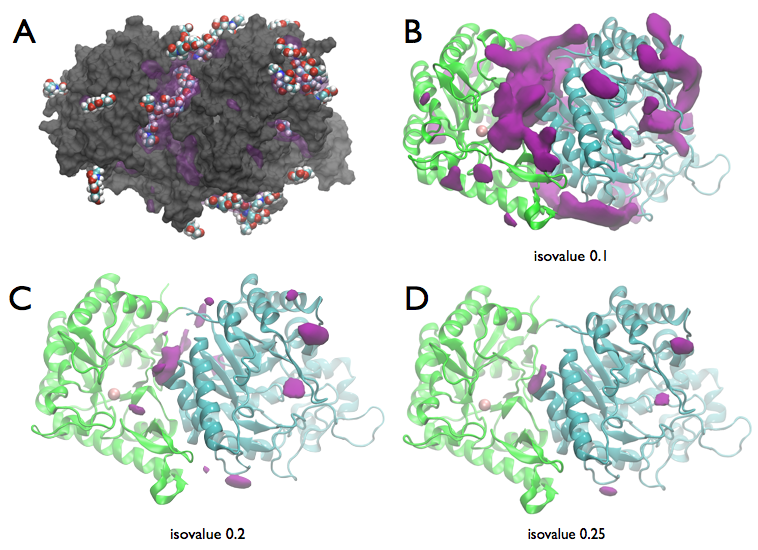
\includegraphics[height=4.25in, width=6in]{figures/results4/figure_pgab_density.png}
%\caption[NAG binding density]{Spatial binding probability density map of bound GlcNAc around PgaB. (A) An example snapshot of PgaB (grey) shown using a surface representation with bound GlcNAc binding density depicted in purple at 10\% occupancy (iso-contour of 0.1). Binding densities of GlcNAc overlapped with a cartoon representation of PgaB at iso-contour levels of (B) 0.1 (C) 0.2 (D) 0.25. In our coloring scheme, residue numbers 43 to 310 and numbers 311 to 667 represent N- (green) and C-terminal (cyan) domains, respectively.}
%\label{fig:pgab_density}
%\end{figure}

%\begin{figure}[htbp]
%\centering
%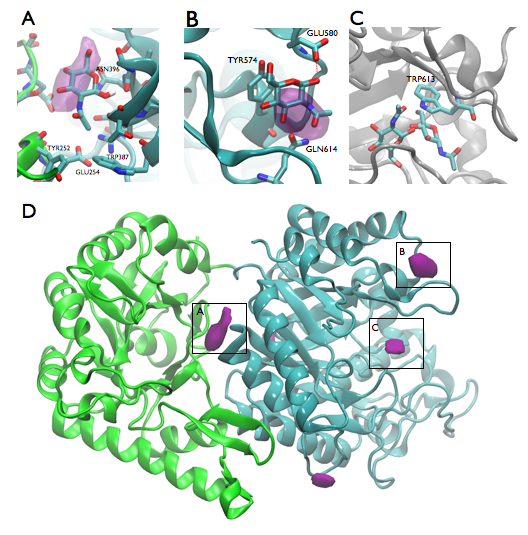
\includegraphics[height=6.29in, width=6.12in]{figures/results4/figure_pgab_binding_sites.png}
%\caption[GlcNAc binding sites]{High probability GlcNAc binding sites at an iso-contour value of 0.25 (D). Insets (A to C) show detailed views of the binding sites and the residues involved in binding. \textbf{This figure probably isn't that useful}}
%\label{fig:pgab_binding_sites}
%\end{figure}

\begin{singlespace}
\addcontentsline{toc}{section}{Bibliography}
\bibliographystyle{elsart-num}
\bibliography{results4/results4}
\end{singlespace}
